\documentclass[10pt]{article}
\usepackage[margin=2cm]{geometry}
\usepackage{graphicx,amsmath,amssymb}
\usepackage[hidelinks]{hyperref}
\graphicspath{{../figures/}{../schematics/}{../layout/png/}}
\newcommand{\mapeIdVgMin}{1.3}
\newcommand{\mapeIdVgMax}{12.1}
\newcommand{\mapeIdVdMin}{3.7}
\newcommand{\mapeIdVdMax}{12.6}
\newcommand{\frosi}{19.39}
\newcommand{\tpdsi}{5.2}
\newcommand{\ecycsi}{2.09}
\newcommand{\pavgsi}{40.6}
\newcommand{\vmsi}{0.49}
\newcommand{\gainsi}{16}
\newcommand{\nmlsi}{0.41}
\newcommand{\nmhsi}{0.44}
\newcommand{\pdpsi}{0.209}
\newcommand{\yfsi}{nan}
\newcommand{\yfuncsi}{nan}
\newcommand{\sigfsi}{nan}
\newcommand{\frosige}{21.39}
\newcommand{\tpdsige}{4.7}
\newcommand{\ecycsige}{2.12}
\newcommand{\pavgsige}{45.4}
\newcommand{\vmsige}{0.49}
\newcommand{\gainsige}{16}
\newcommand{\nmlsige}{0.42}
\newcommand{\nmhsige}{0.43}
\newcommand{\pdpsige}{0.212}
\newcommand{\yfsige}{nan}
\newcommand{\yfuncsige}{nan}
\newcommand{\sigfsige}{nan}
\newcommand{\frotmd}{2.59}
\newcommand{\tpdtmd}{38.7}
\newcommand{\ecyctmd}{0.67}
\newcommand{\pavgtmd}{1.7}
\newcommand{\vmtmd}{0.48}
\newcommand{\gaintmd}{12}
\newcommand{\nmltmd}{0.41}
\newcommand{\nmhtmd}{0.45}
\newcommand{\pdptmd}{0.067}
\newcommand{\yftmd}{nan}
\newcommand{\yfunctmd}{nan}
\newcommand{\sigftmd}{nan}
\newcommand{\frocnt}{45.39}
\newcommand{\tpdcnt}{2.2}
\newcommand{\ecyccnt}{0.84}
\newcommand{\pavgcnt}{38.0}
\newcommand{\vmcnt}{0.50}
\newcommand{\gaincnt}{22}
\newcommand{\nmlcnt}{0.42}
\newcommand{\nmhcnt}{0.41}
\newcommand{\pdpcnt}{0.084}
\newcommand{\yfcnt}{nan}
\newcommand{\yfunccnt}{nan}
\newcommand{\sigfcnt}{nan}
\newcommand{\frogan}{1.69}
\newcommand{\tpdgan}{59.1}
\newcommand{\ecycgan}{94.17}
\newcommand{\pavggan}{159.4}
\newcommand{\vmgan}{0.42}
\newcommand{\gaingan}{18}
\newcommand{\nmlgan}{0.25}
\newcommand{\nmhgan}{0.49}
\newcommand{\pdpgan}{9.417}
\newcommand{\yfgan}{nan}
\newcommand{\yfuncgan}{nan}
\newcommand{\sigfgan}{nan}
\newcommand{\tcfgan}{nan}
\newcommand{\fFiveHundredgan}{nan}
\newcommand{\tcfsi}{nan}
\newcommand{\fFiveHundredsi}{nan}
\newcommand{\areainvcfetsi}{8640}
\newcommand{\arearoFivecfetsi}{54000}
\newcommand{\areainvcfetsige}{8640}
\newcommand{\arearoFivecfetsige}{54000}
\newcommand{\areainvcfettmd}{10368}
\newcommand{\arearoFivecfettmd}{64800}
\newcommand{\areainvcfetcnt}{10368}
\newcommand{\arearoFivecfetcnt}{64800}
\newcommand{\areainvcfetgan}{160000}
\newcommand{\arearoFivecfetgan}{1000000}

\newcommand{\ucm}{UCM-CFET}
\pagestyle{plain}
\begin{document}
\begin{center}\Large\bfseries Figures\\[2pt]\normalsize\mdseries A Unified Physics-Based Compact Model and Calibrated Circuit-Validation Flow for Multi-Material CFET Logic: Si, SiGe, MoS$_2$/WSe$_2$, CNT and GaN\\[4pt]\small M. Nisha Angeline\end{center}
\vspace{4pt}\noindent All figures are also provided as individual PNG (300 dpi) and PDF files in \texttt{figures/}, \texttt{schematics/} and \texttt{layout/png/}.
\clearpage
\begin{figure}[p]\centering
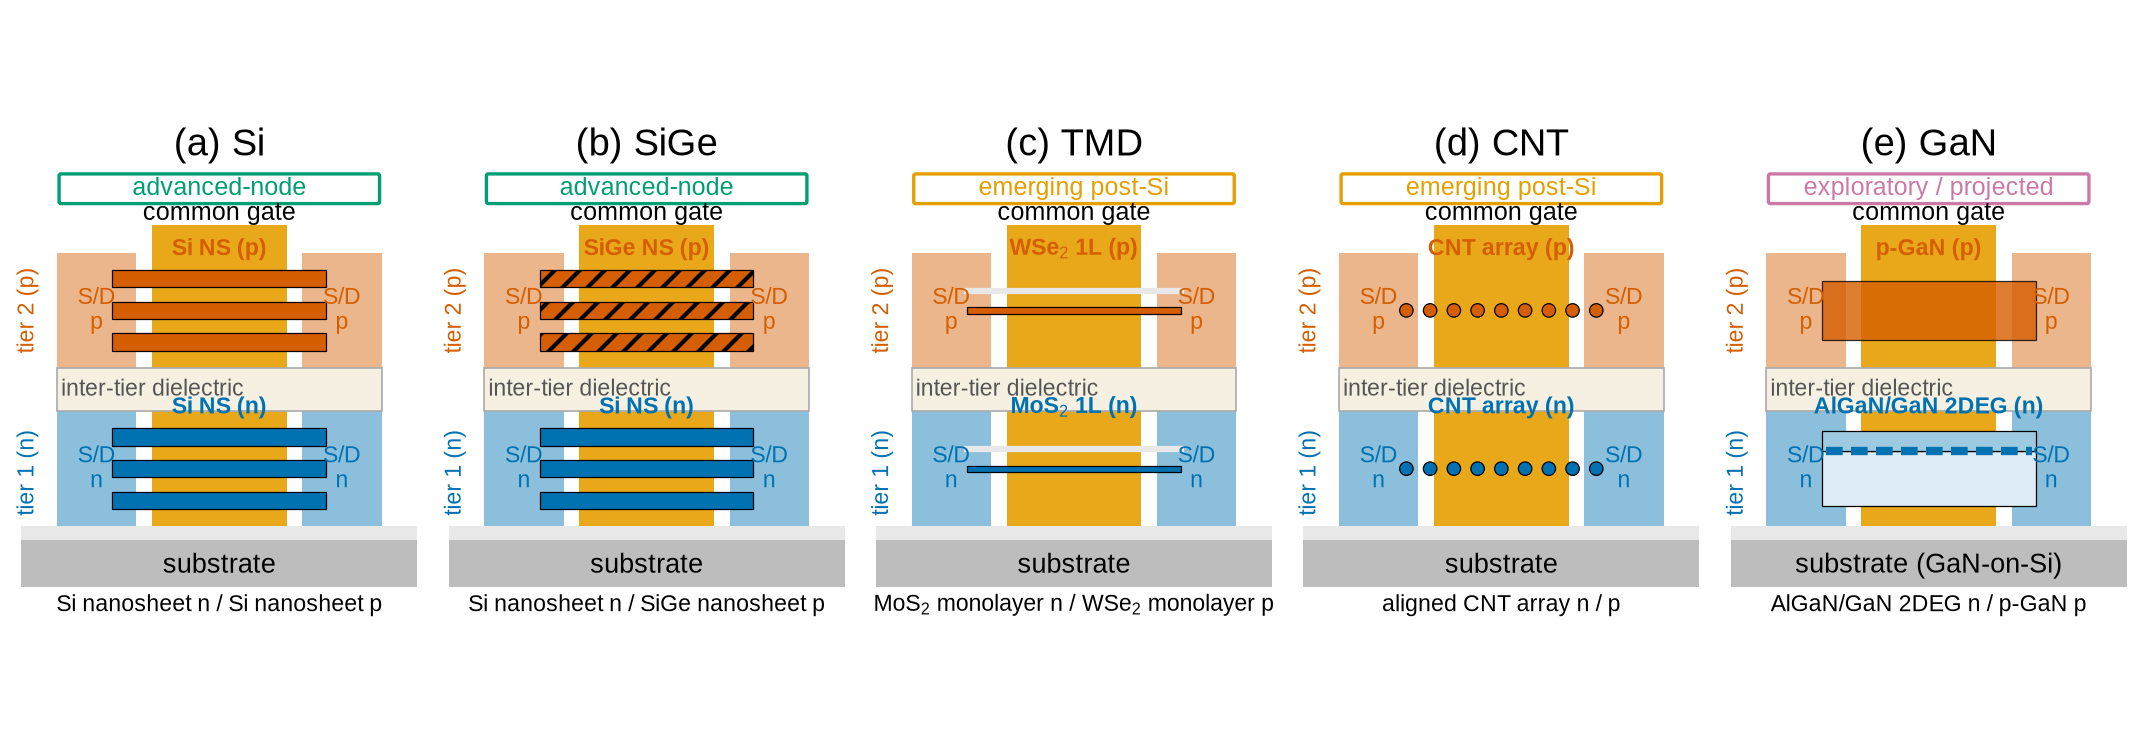
\includegraphics[width=\textwidth,height=0.82\textheight,keepaspectratio]{fig01_cfet_stacks.png}
\par\vspace{6pt}\noindent\textbf{Fig.~1.} Cross-section cartoons of the five CFET platforms: bottom n-tier, inter-tier dielectric, top p-tier, common gate wrapping both tiers, and n/p source/drain contacts. Maturity tags follow Table~I.
\end{figure}\clearpage
\begin{figure}[p]\centering
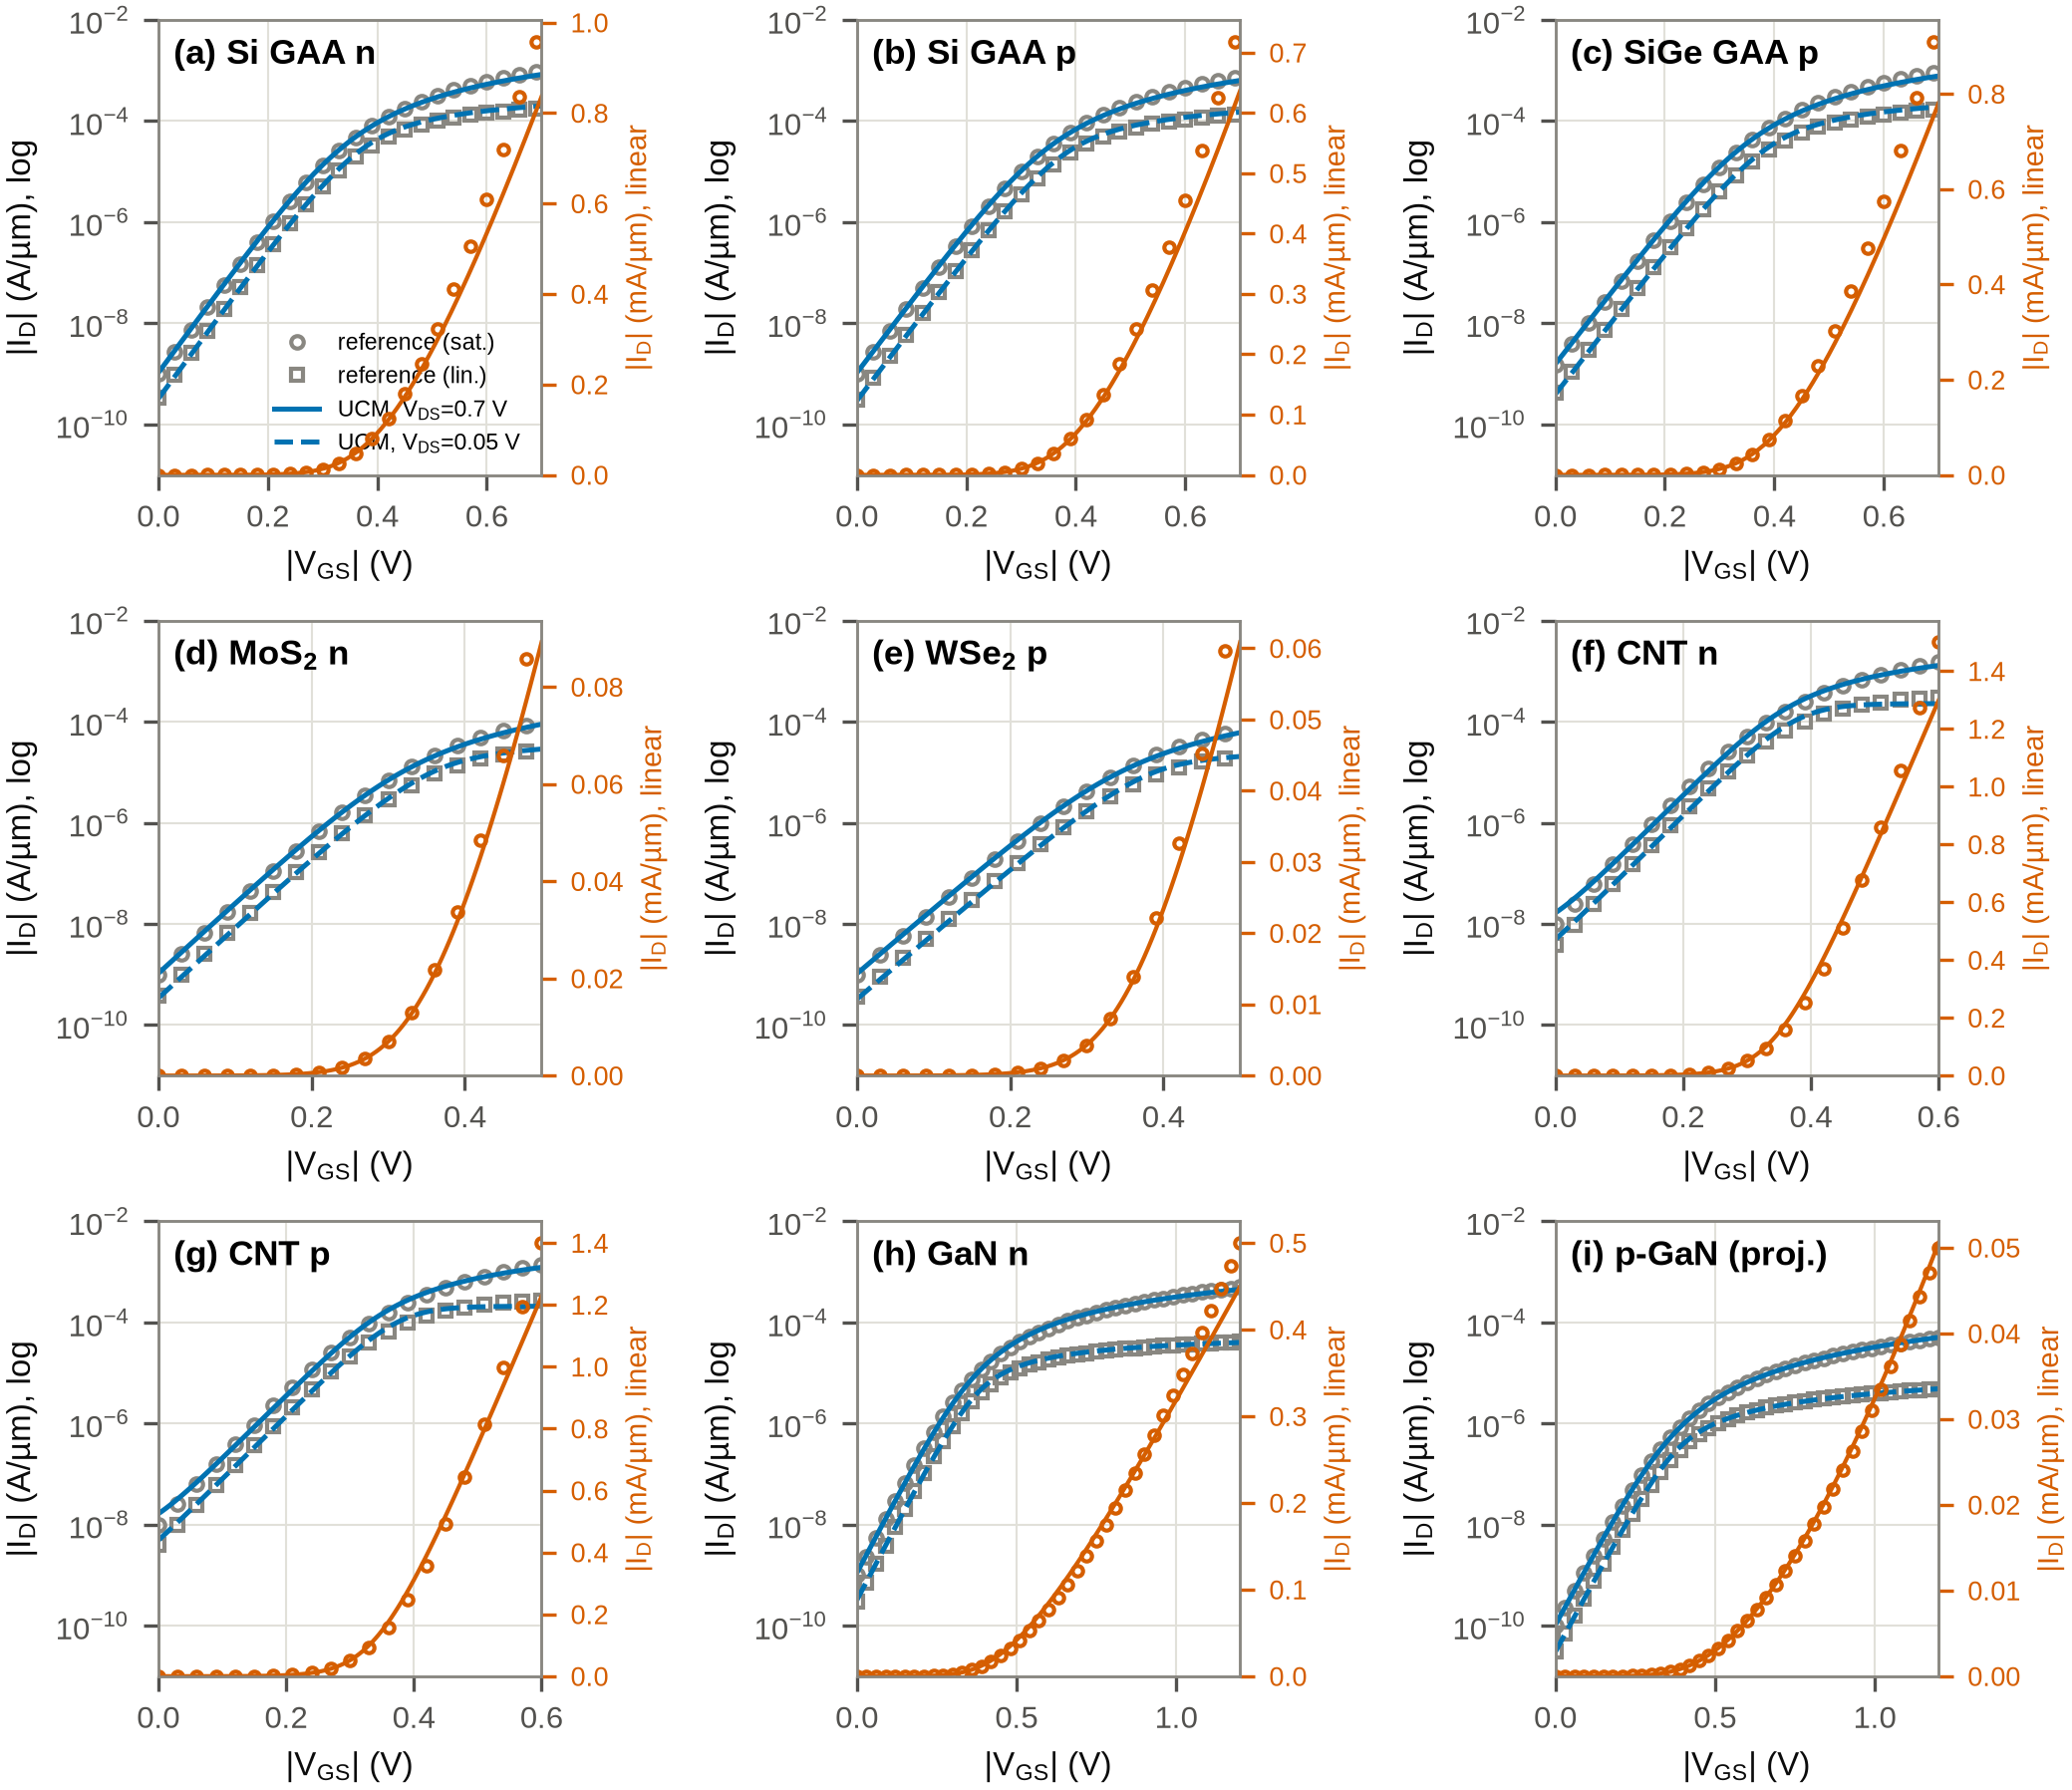
\includegraphics[width=\textwidth,height=0.82\textheight,keepaspectratio]{fig02_calibration_idvg.png}
\par\vspace{6pt}\noindent\textbf{Fig.~2.} $I_D$--$V_G$ calibration of the nine device models (lines) against the literature-anchored reference curves (symbols) at $|V_{DS}|=0.05$~V and $|V_{DS}|=V_{DD}$, on logarithmic (left axes) and linear (right axes) scales.
\end{figure}\clearpage
\begin{figure}[p]\centering
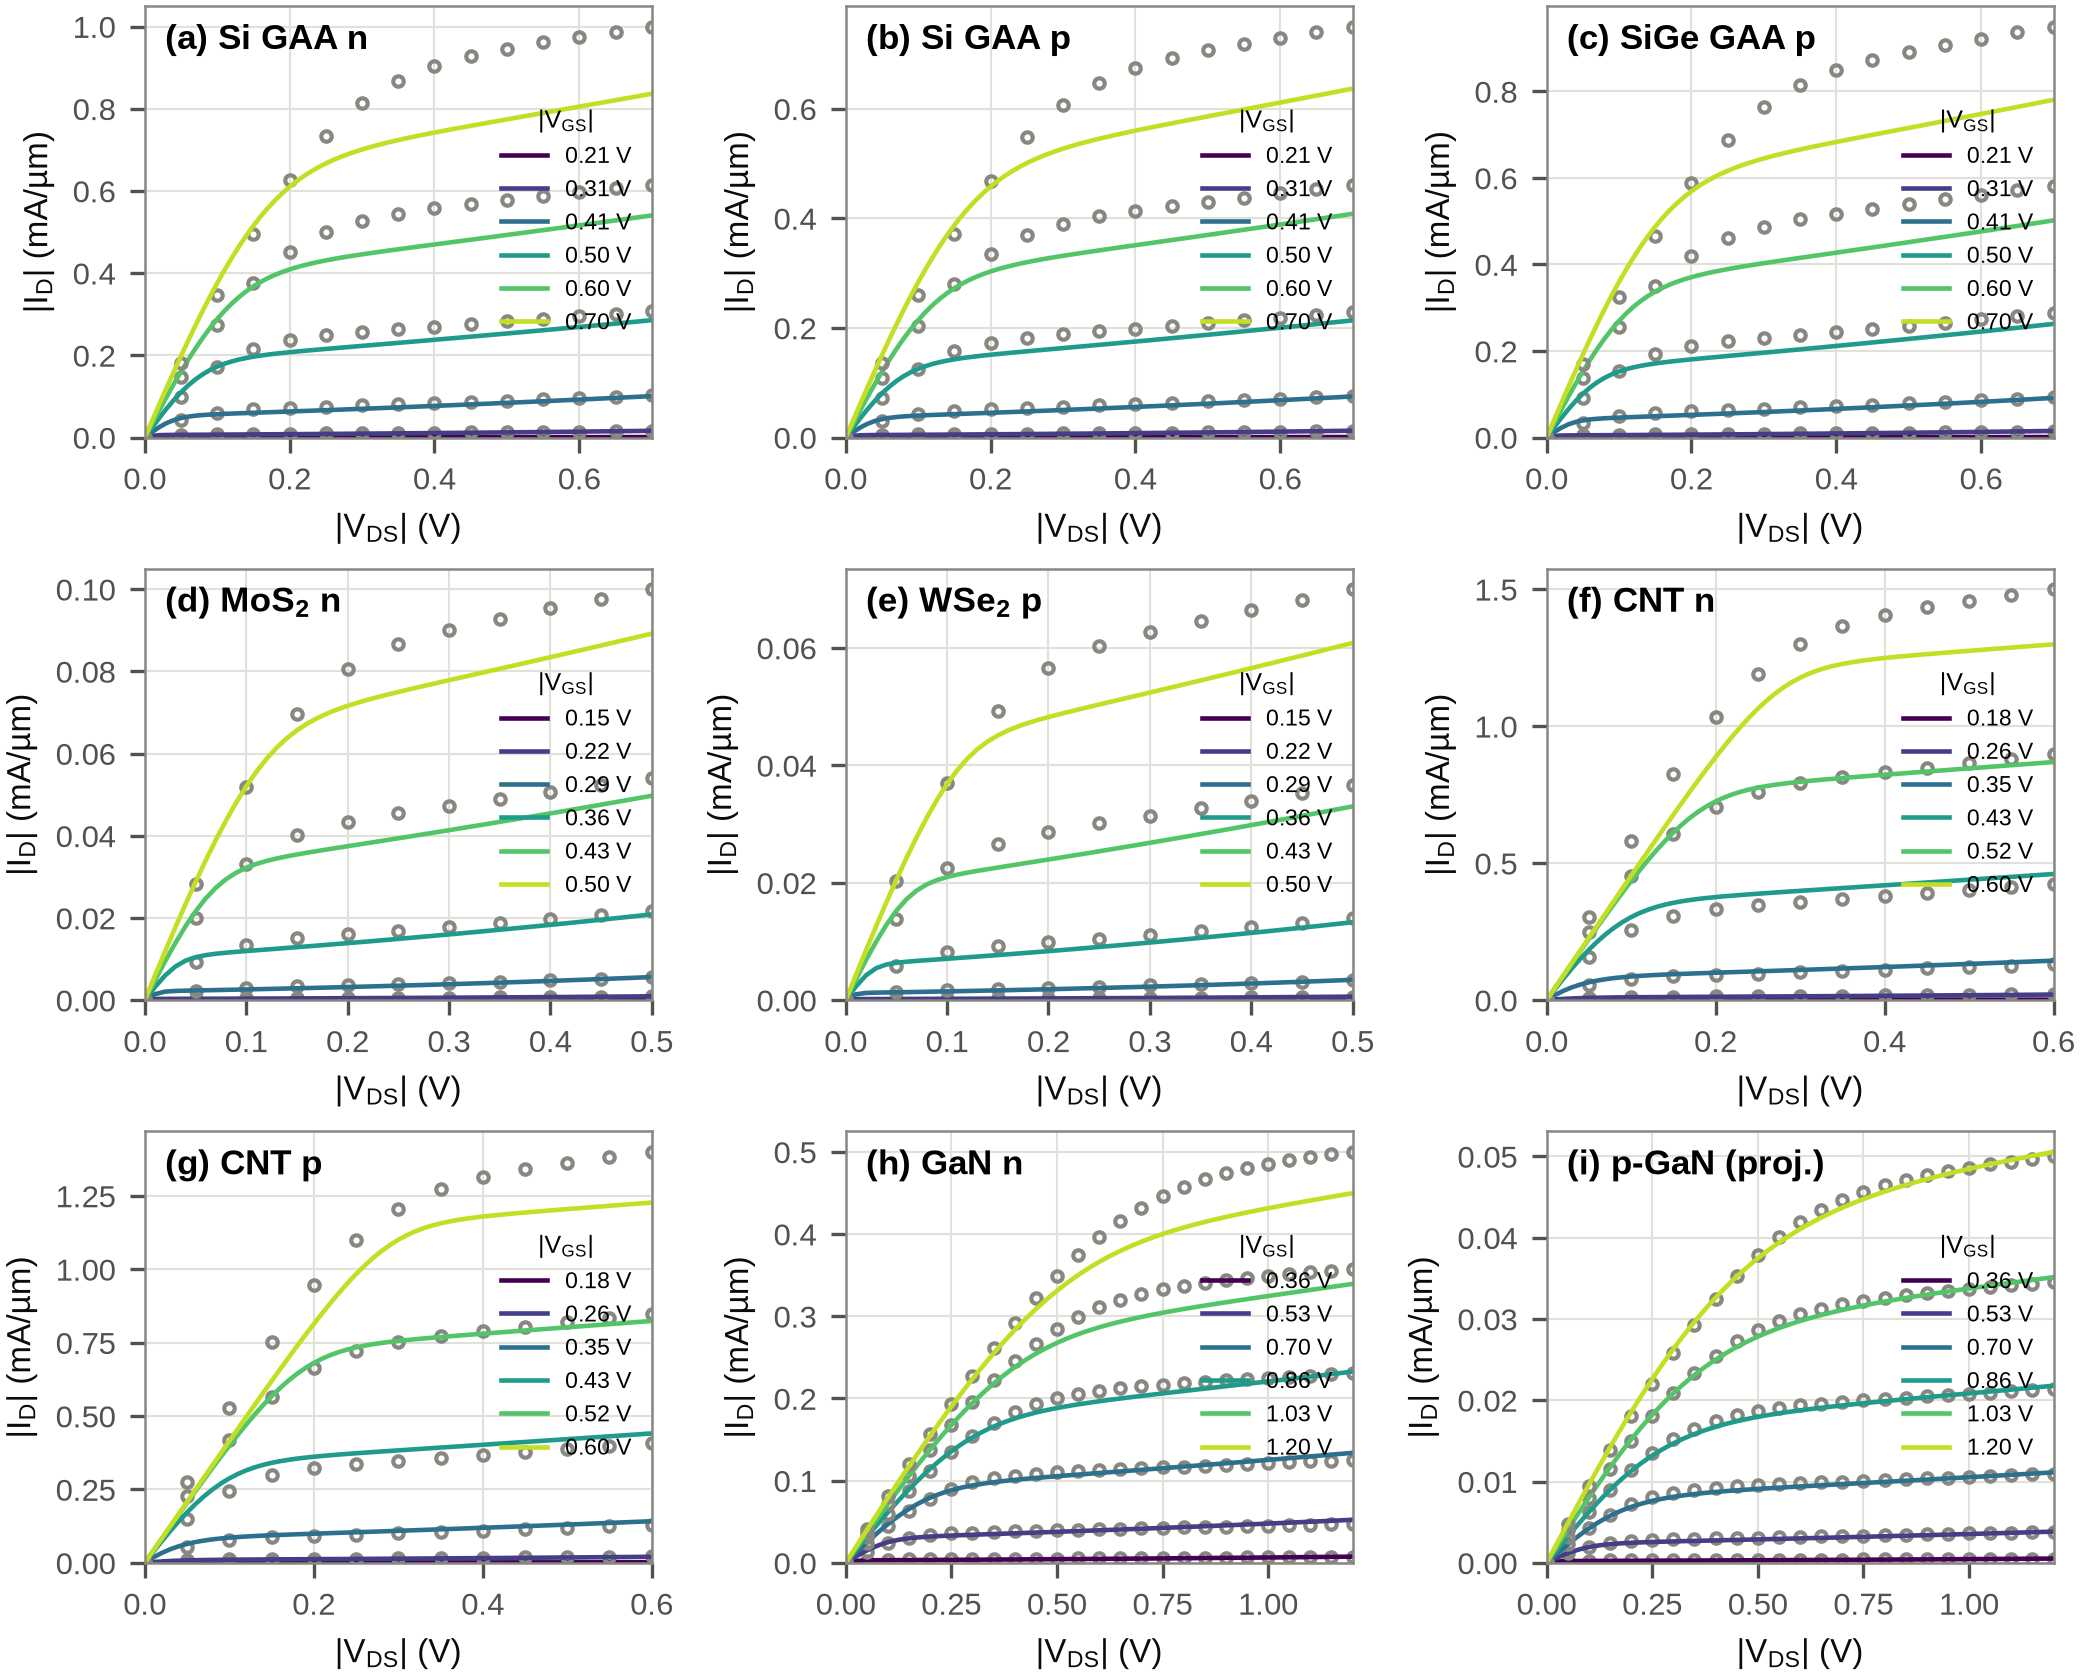
\includegraphics[width=\textwidth,height=0.82\textheight,keepaspectratio]{fig03_calibration_idvd.png}
\par\vspace{6pt}\noindent\textbf{Fig.~3.} $I_D$--$V_D$ families (six gate biases from $0.3V_{DD}$ to $V_{DD}$) of the calibrated models (lines) and reference (symbols).
\end{figure}\clearpage
\begin{figure}[p]\centering
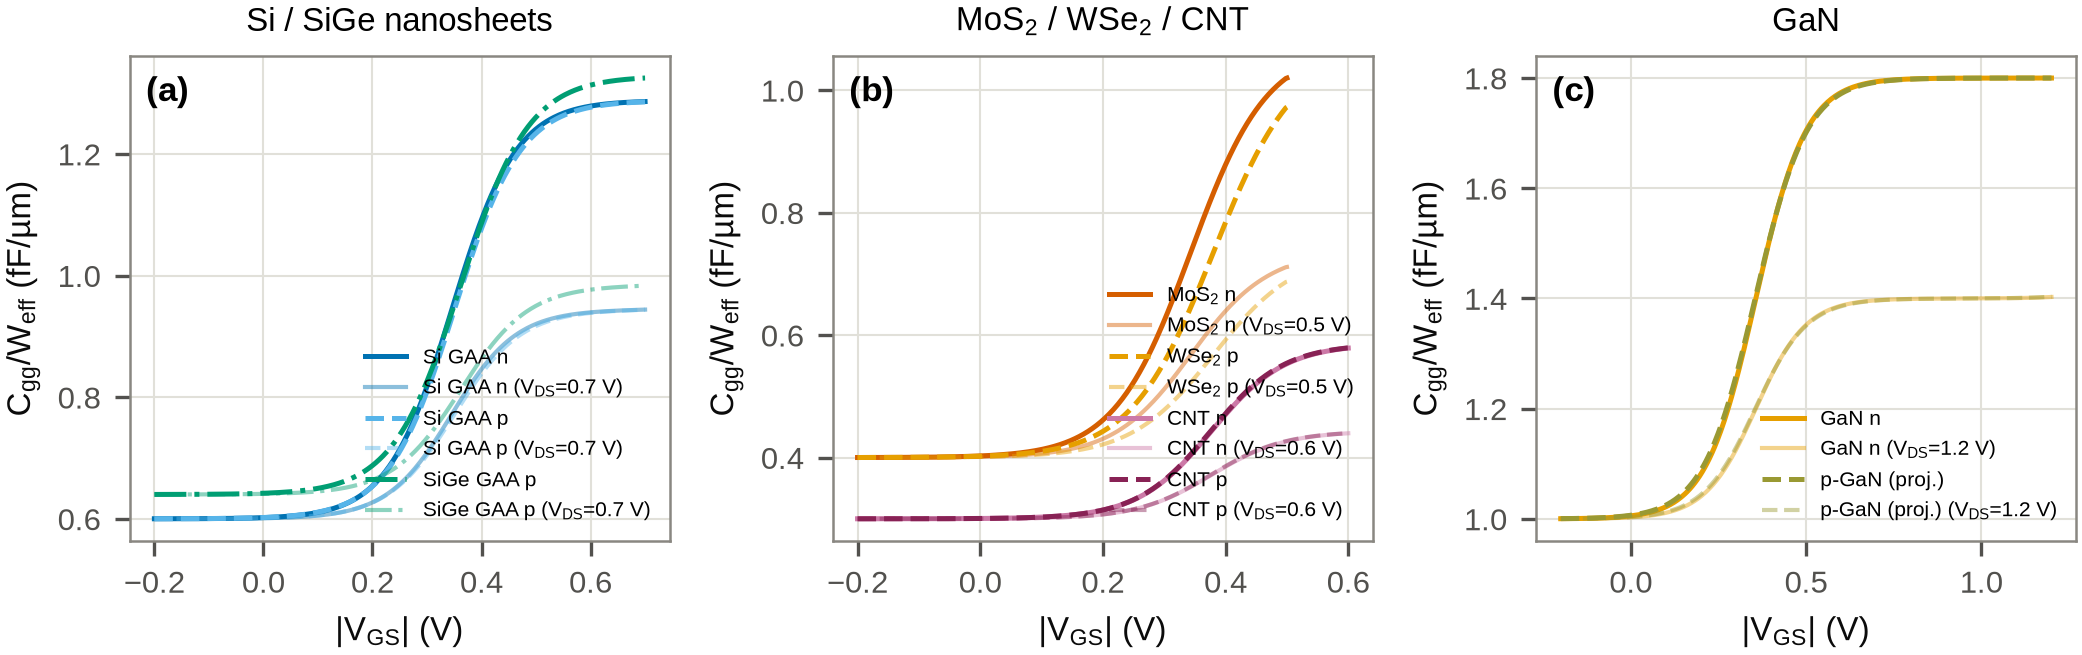
\includegraphics[width=\textwidth,height=0.82\textheight,keepaspectratio]{fig03b_capacitance.png}
\par\vspace{6pt}\noindent\textbf{Fig.~4.} Gate capacitance per effective width, $C_{gg}=\mathrm{d}Q_g/\mathrm{d}V_{GS}$, of the nine calibrated models from the charge model at $V_{DS}=0$ (full lines) and $V_{DS}=V_{DD}$ (faded): (a) Si/SiGe nanosheets, (b) 2D and CNT channels, (c) GaN.
\end{figure}\clearpage
\begin{figure}[p]\centering
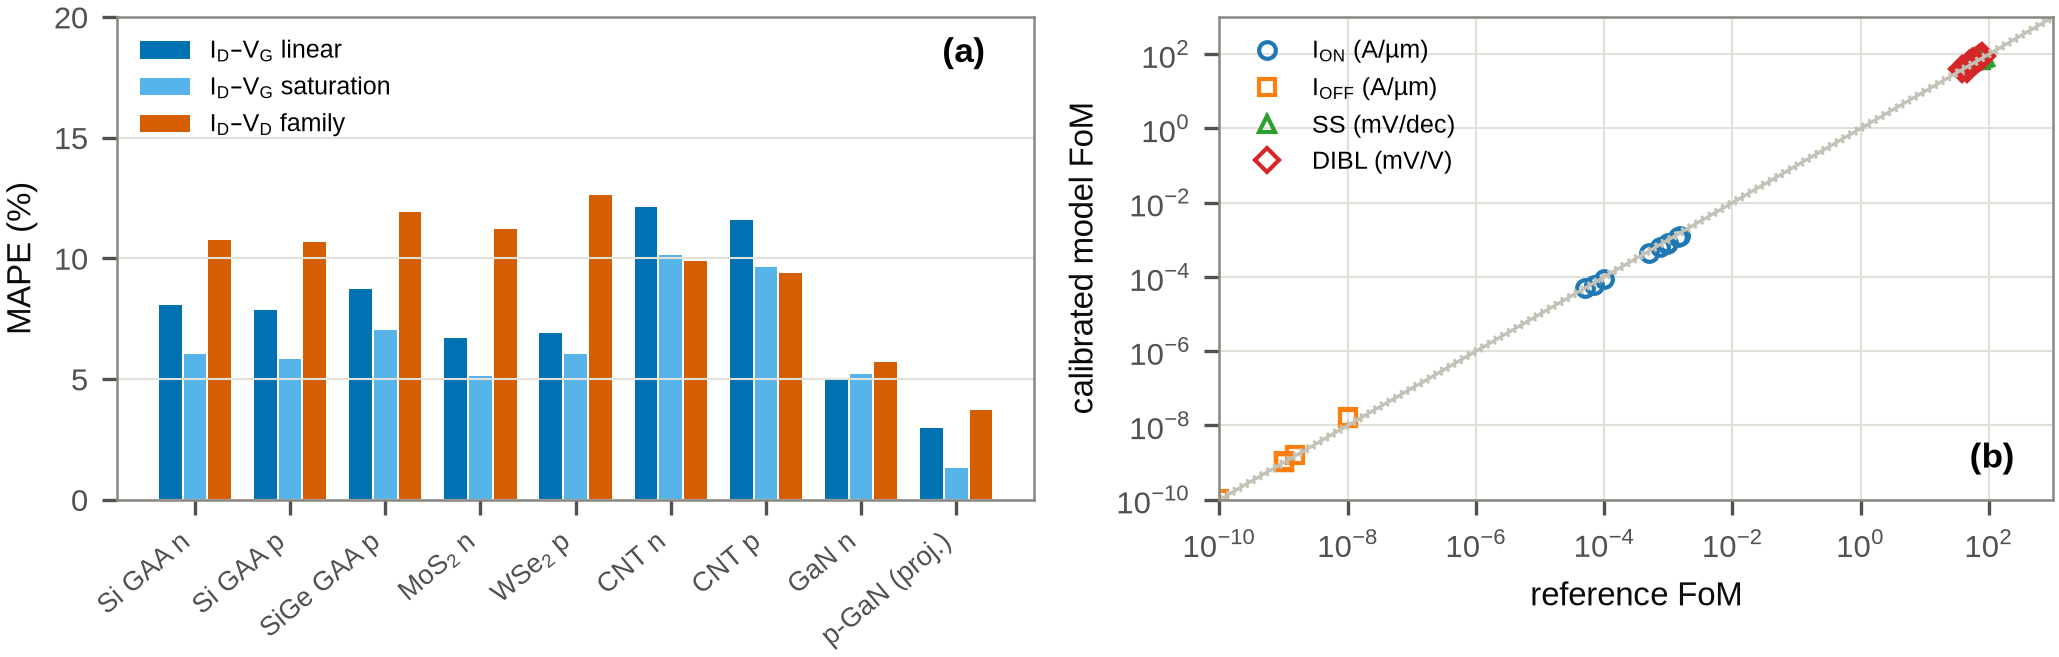
\includegraphics[width=\textwidth,height=0.82\textheight,keepaspectratio]{fig04_calibration_mape.png}
\par\vspace{6pt}\noindent\textbf{Fig.~5.} (a) MAPE per device and data set; (b) parity of model vs. reference figures of merit.
\end{figure}\clearpage
\begin{figure}[p]\centering
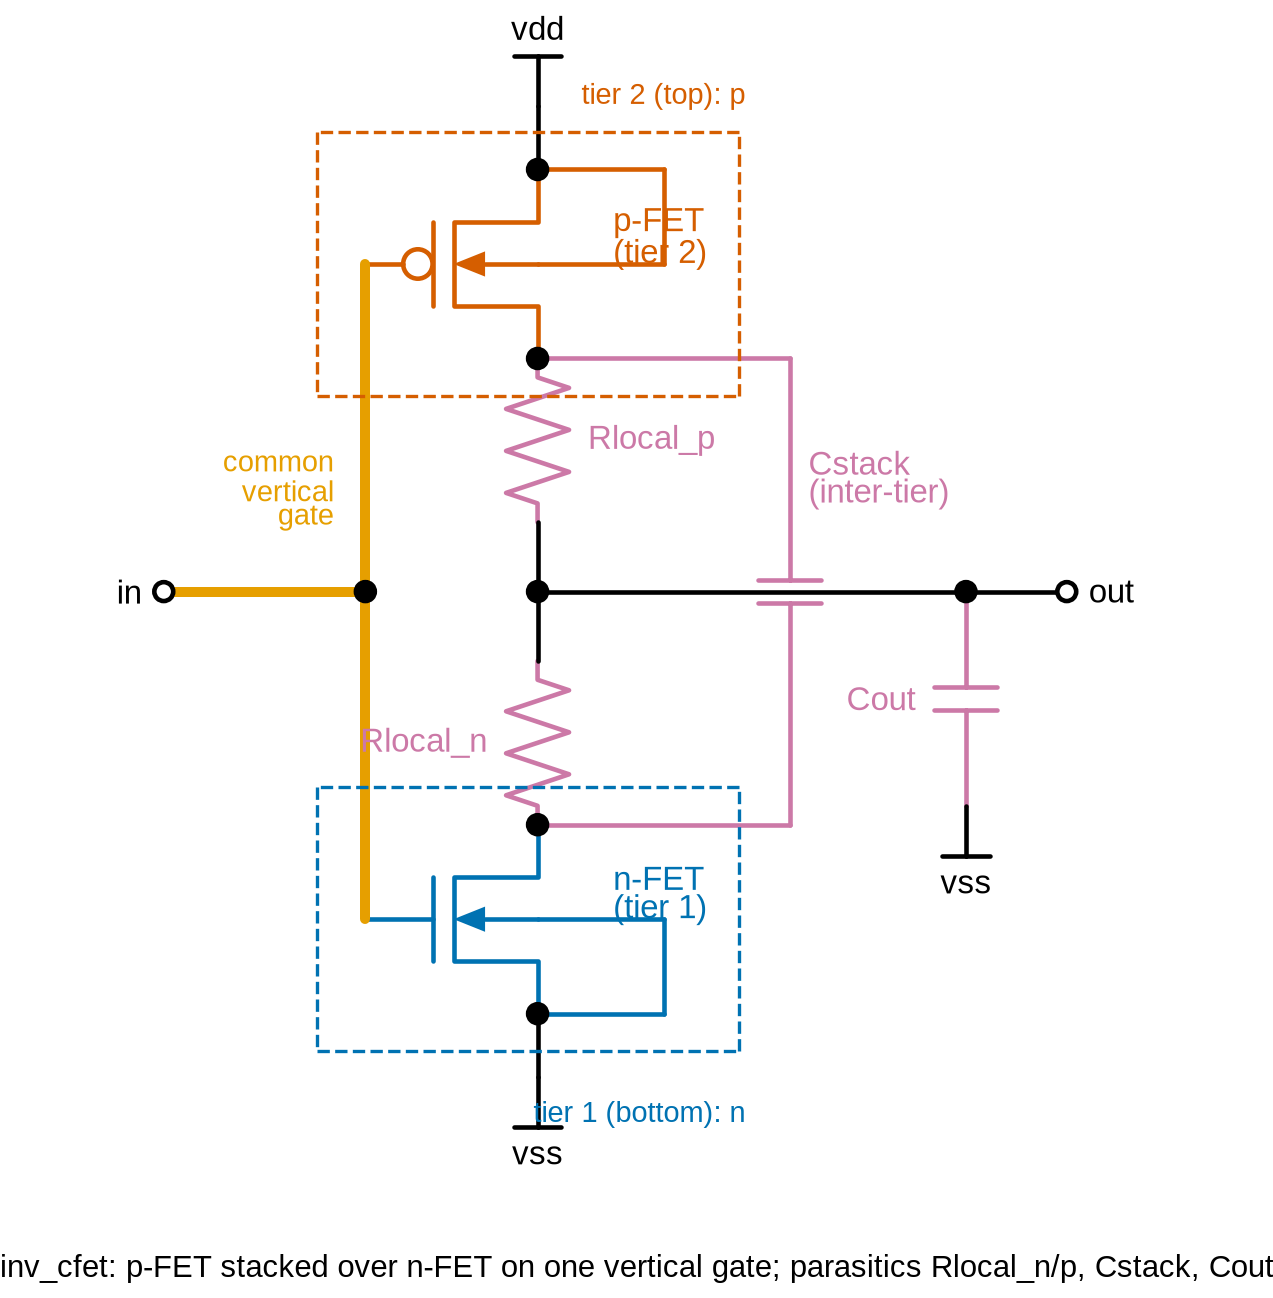
\includegraphics[width=0.48\textwidth]{inv_cfet.png}\hfill
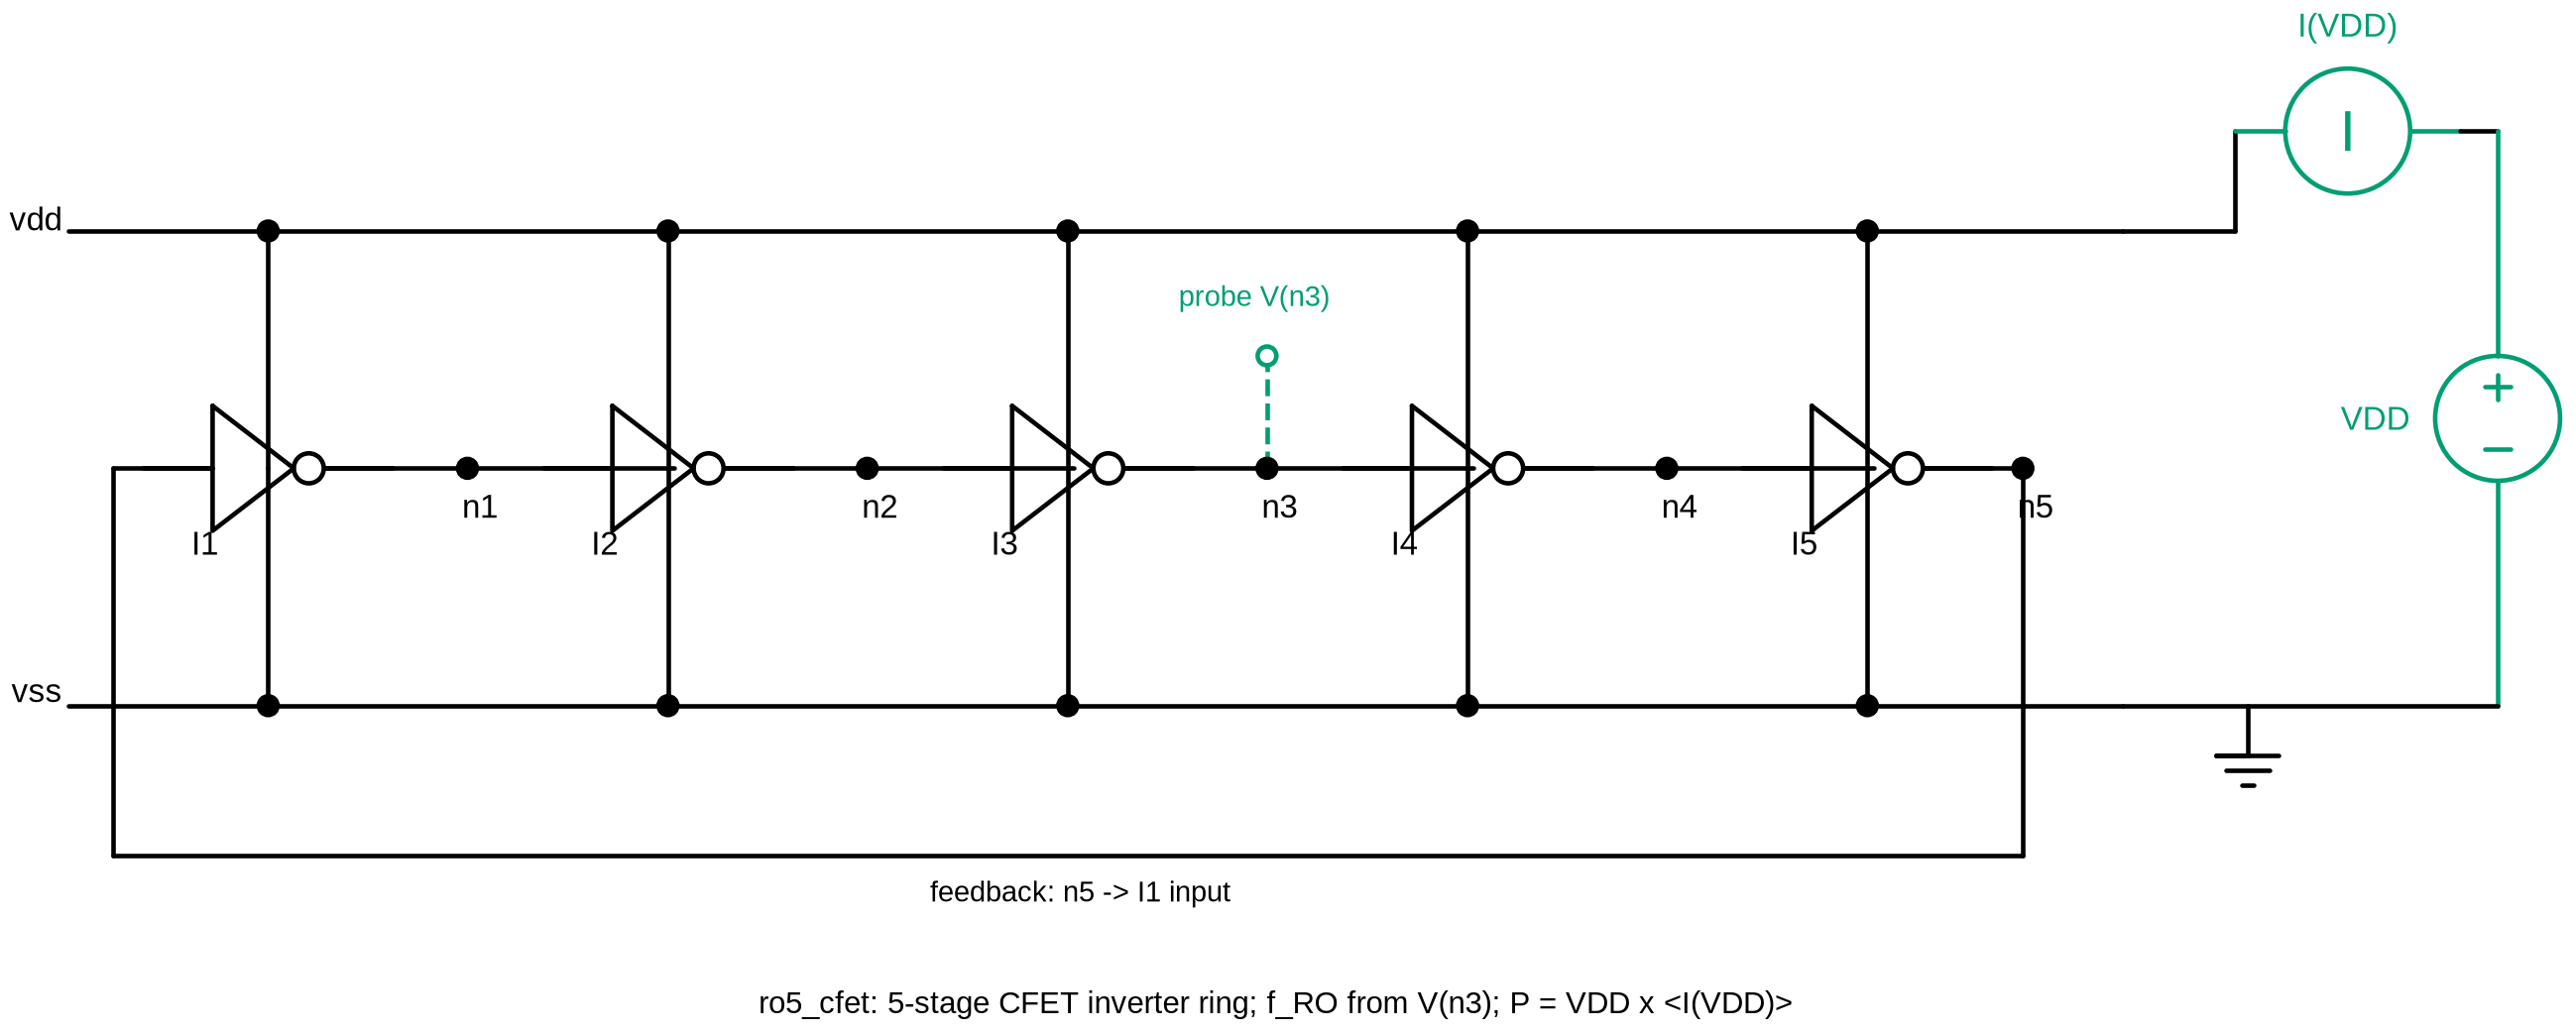
\includegraphics[width=0.48\textwidth]{ro5_cfet.png}
\par\vspace{6pt}\noindent\textbf{Fig.~6.} (a) CFET inverter cell with the explicit inter-tier coupling capacitance $C_{stack}$, output parasitic $C_{out}$ and local-interconnect resistances $R_{local,n/p}$; (b) 5-stage ring oscillator testbench with the $V(n_3)$ probe and the $I(V_{DD})$ meter.
\end{figure}\clearpage
\begin{figure}[p]\centering
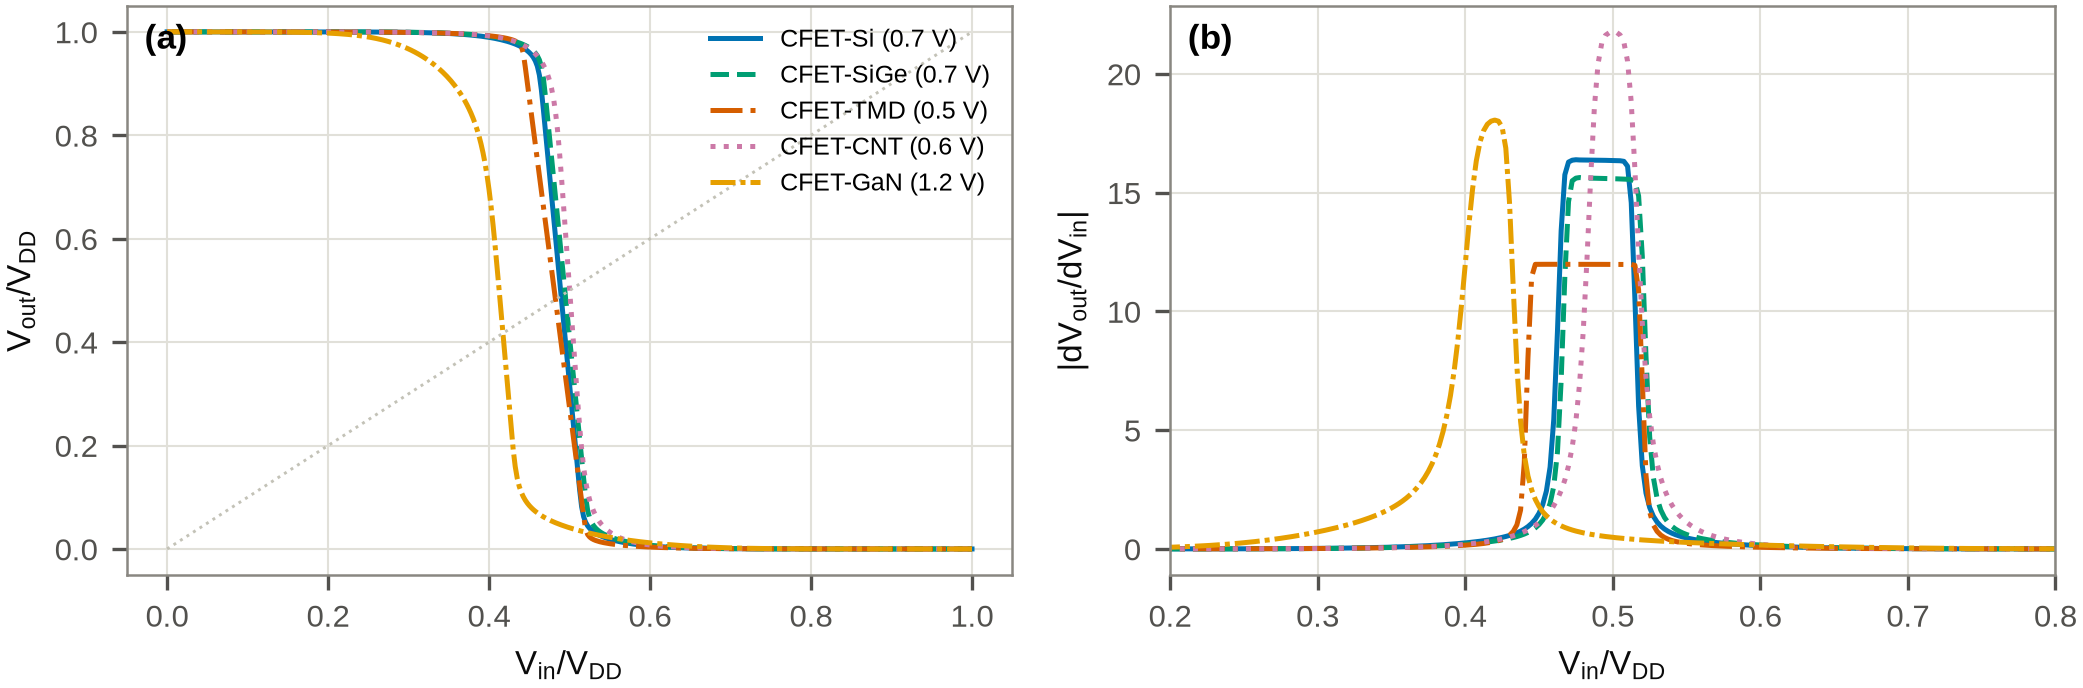
\includegraphics[width=\textwidth,height=0.82\textheight,keepaspectratio]{fig05_inverter_vtc.png}
\par\vspace{6pt}\noindent\textbf{Fig.~7.} (a) Normalised voltage-transfer characteristics of the five CFET inverters at their nominal $V_{DD}$; (b) small-signal gain.
\end{figure}\clearpage
\begin{figure}[p]\centering
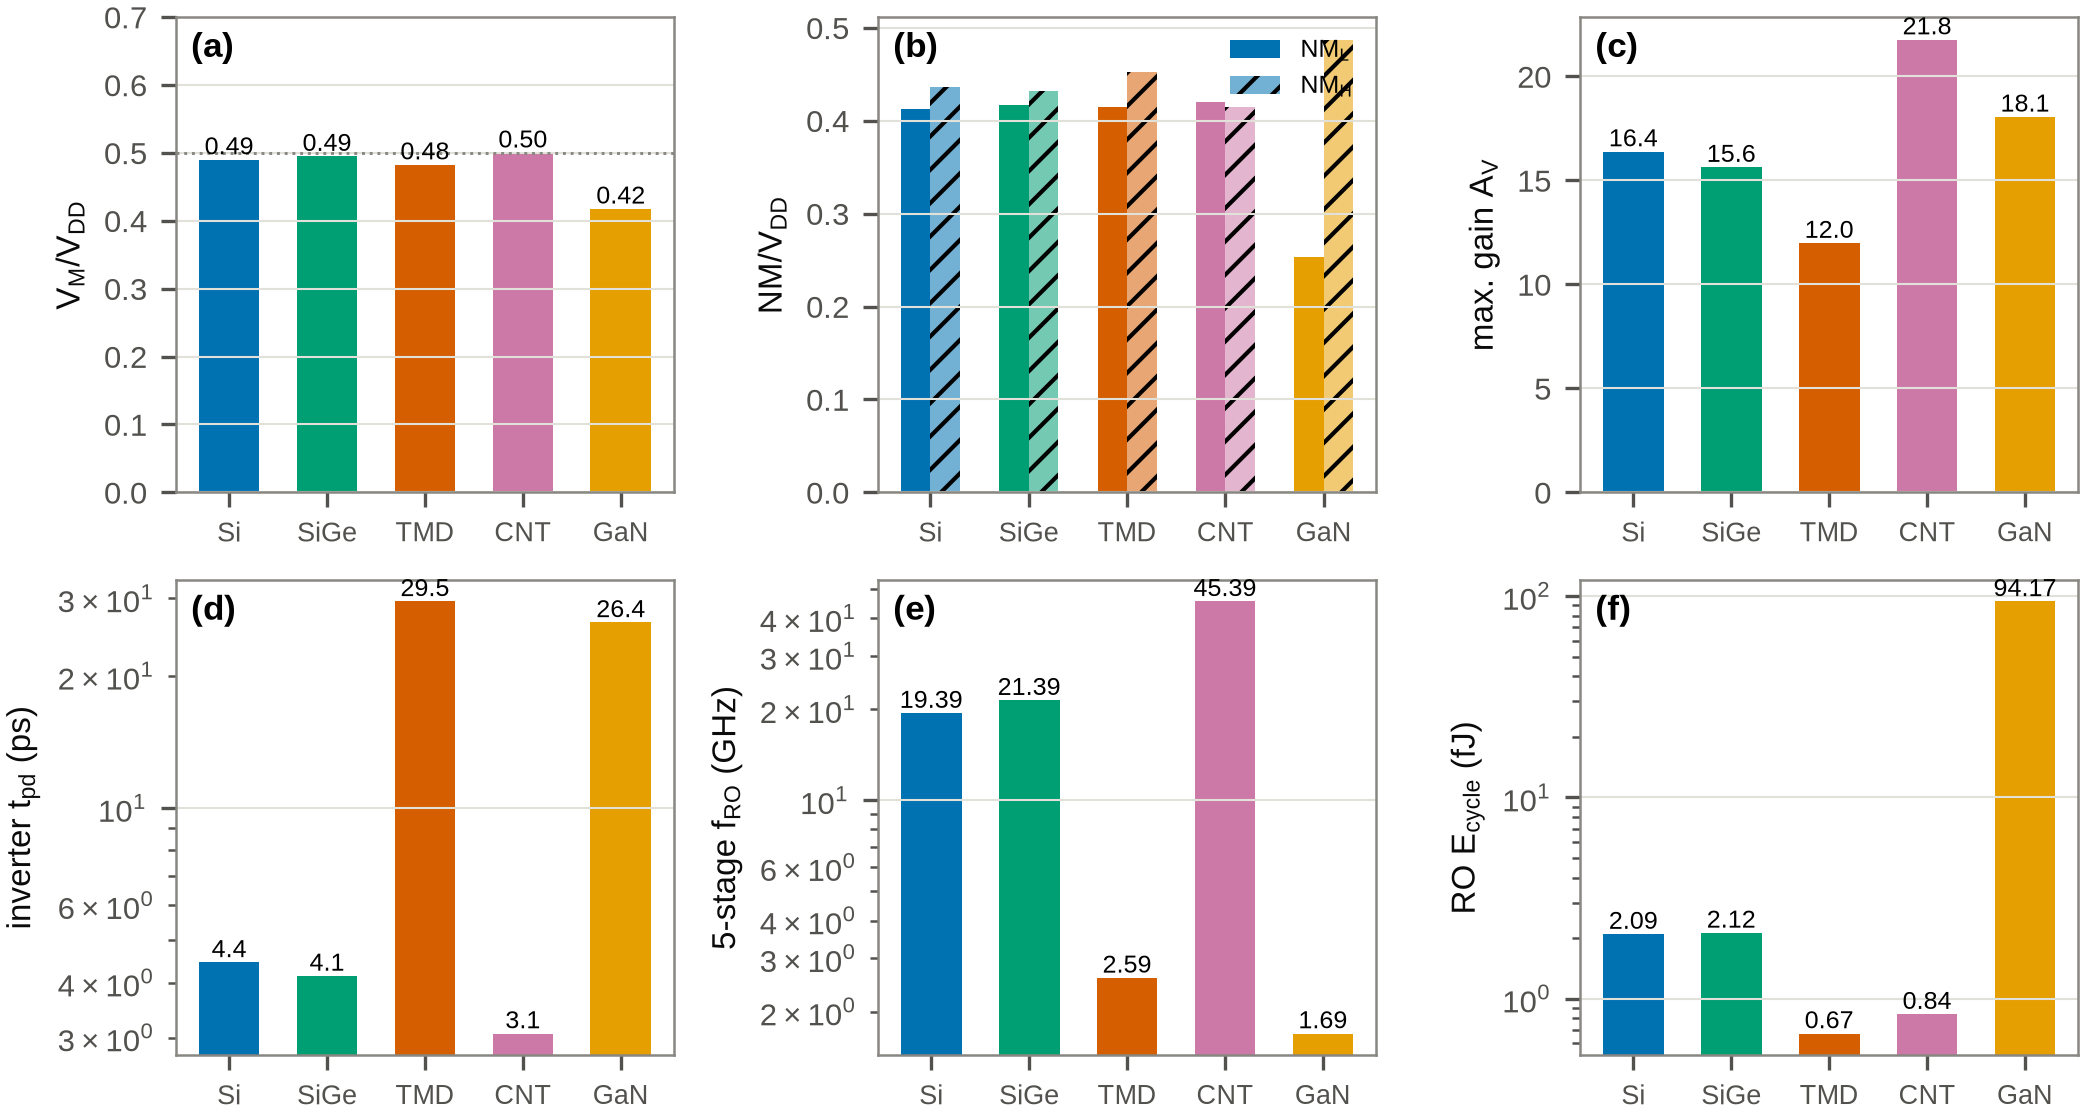
\includegraphics[width=\textwidth,height=0.82\textheight,keepaspectratio]{fig06_inverter_ro_fom.png}
\par\vspace{6pt}\noindent\textbf{Fig.~8.} Nominal figures of merit: (a) $V_M/V_{DD}$, (b) noise margins, (c) maximum gain, (d) inverter delay, (e) 5-stage RO frequency, (f) energy per RO cycle.
\end{figure}\clearpage
\begin{figure}[p]\centering
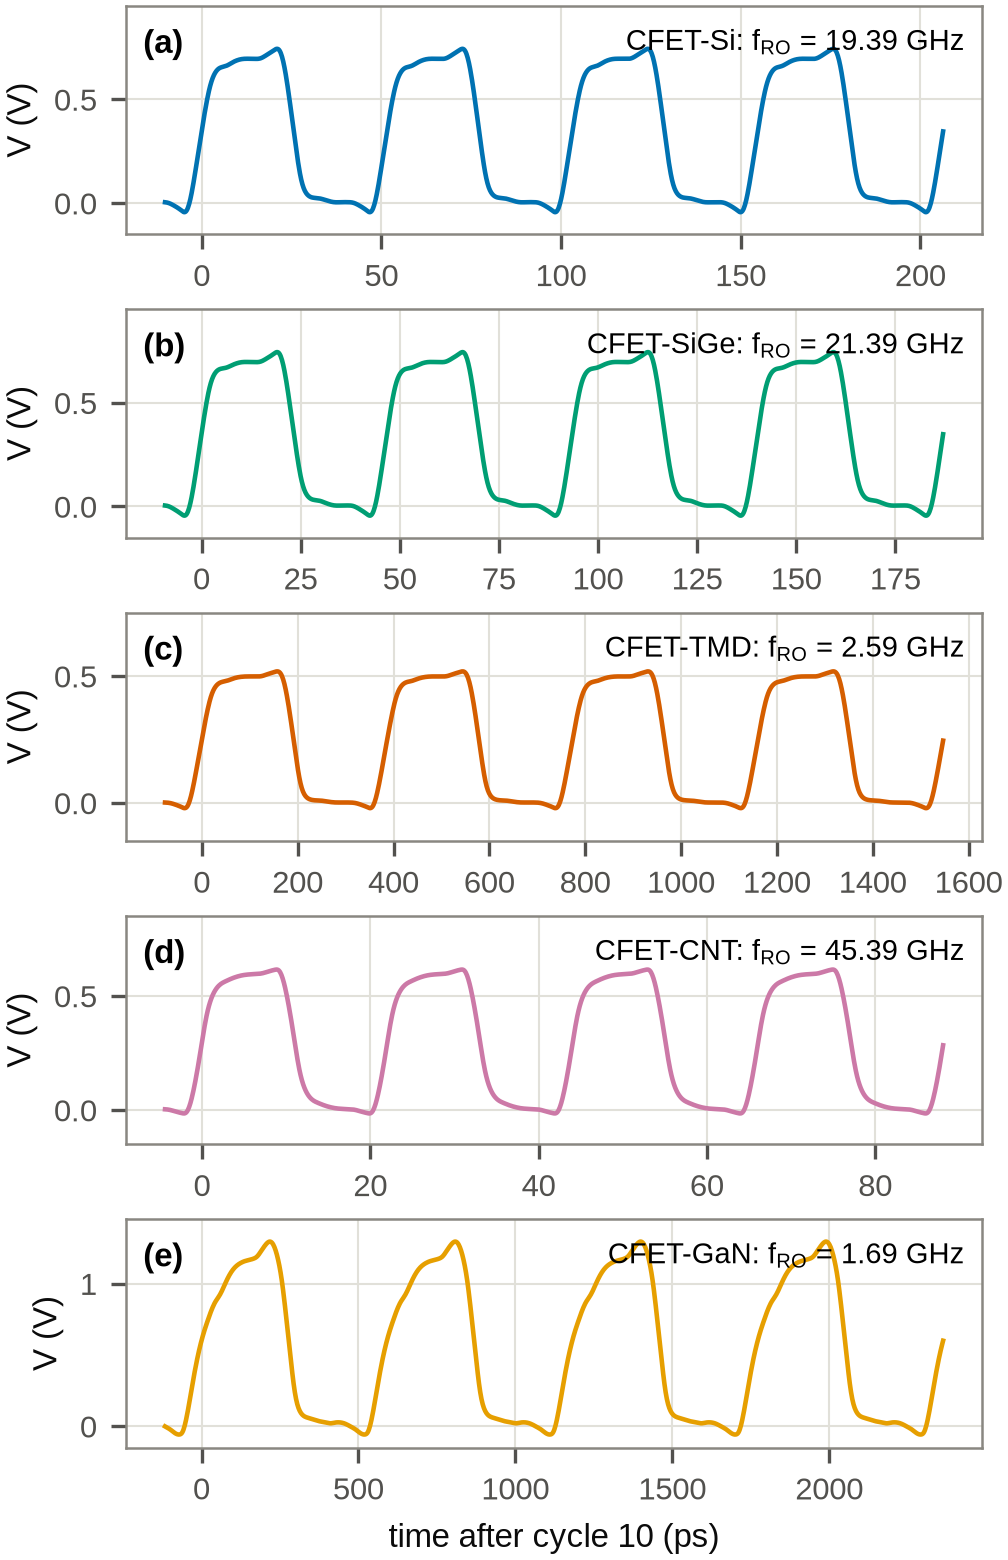
\includegraphics[width=\textwidth,height=0.82\textheight,keepaspectratio]{fig07_ro_waveforms.png}
\par\vspace{6pt}\noindent\textbf{Fig.~9.} 5-stage RO waveforms $V(n_3)$ for the five platforms, four cycles after cycle 10 (the measurement window).
\end{figure}\clearpage
\begin{figure}[p]\centering
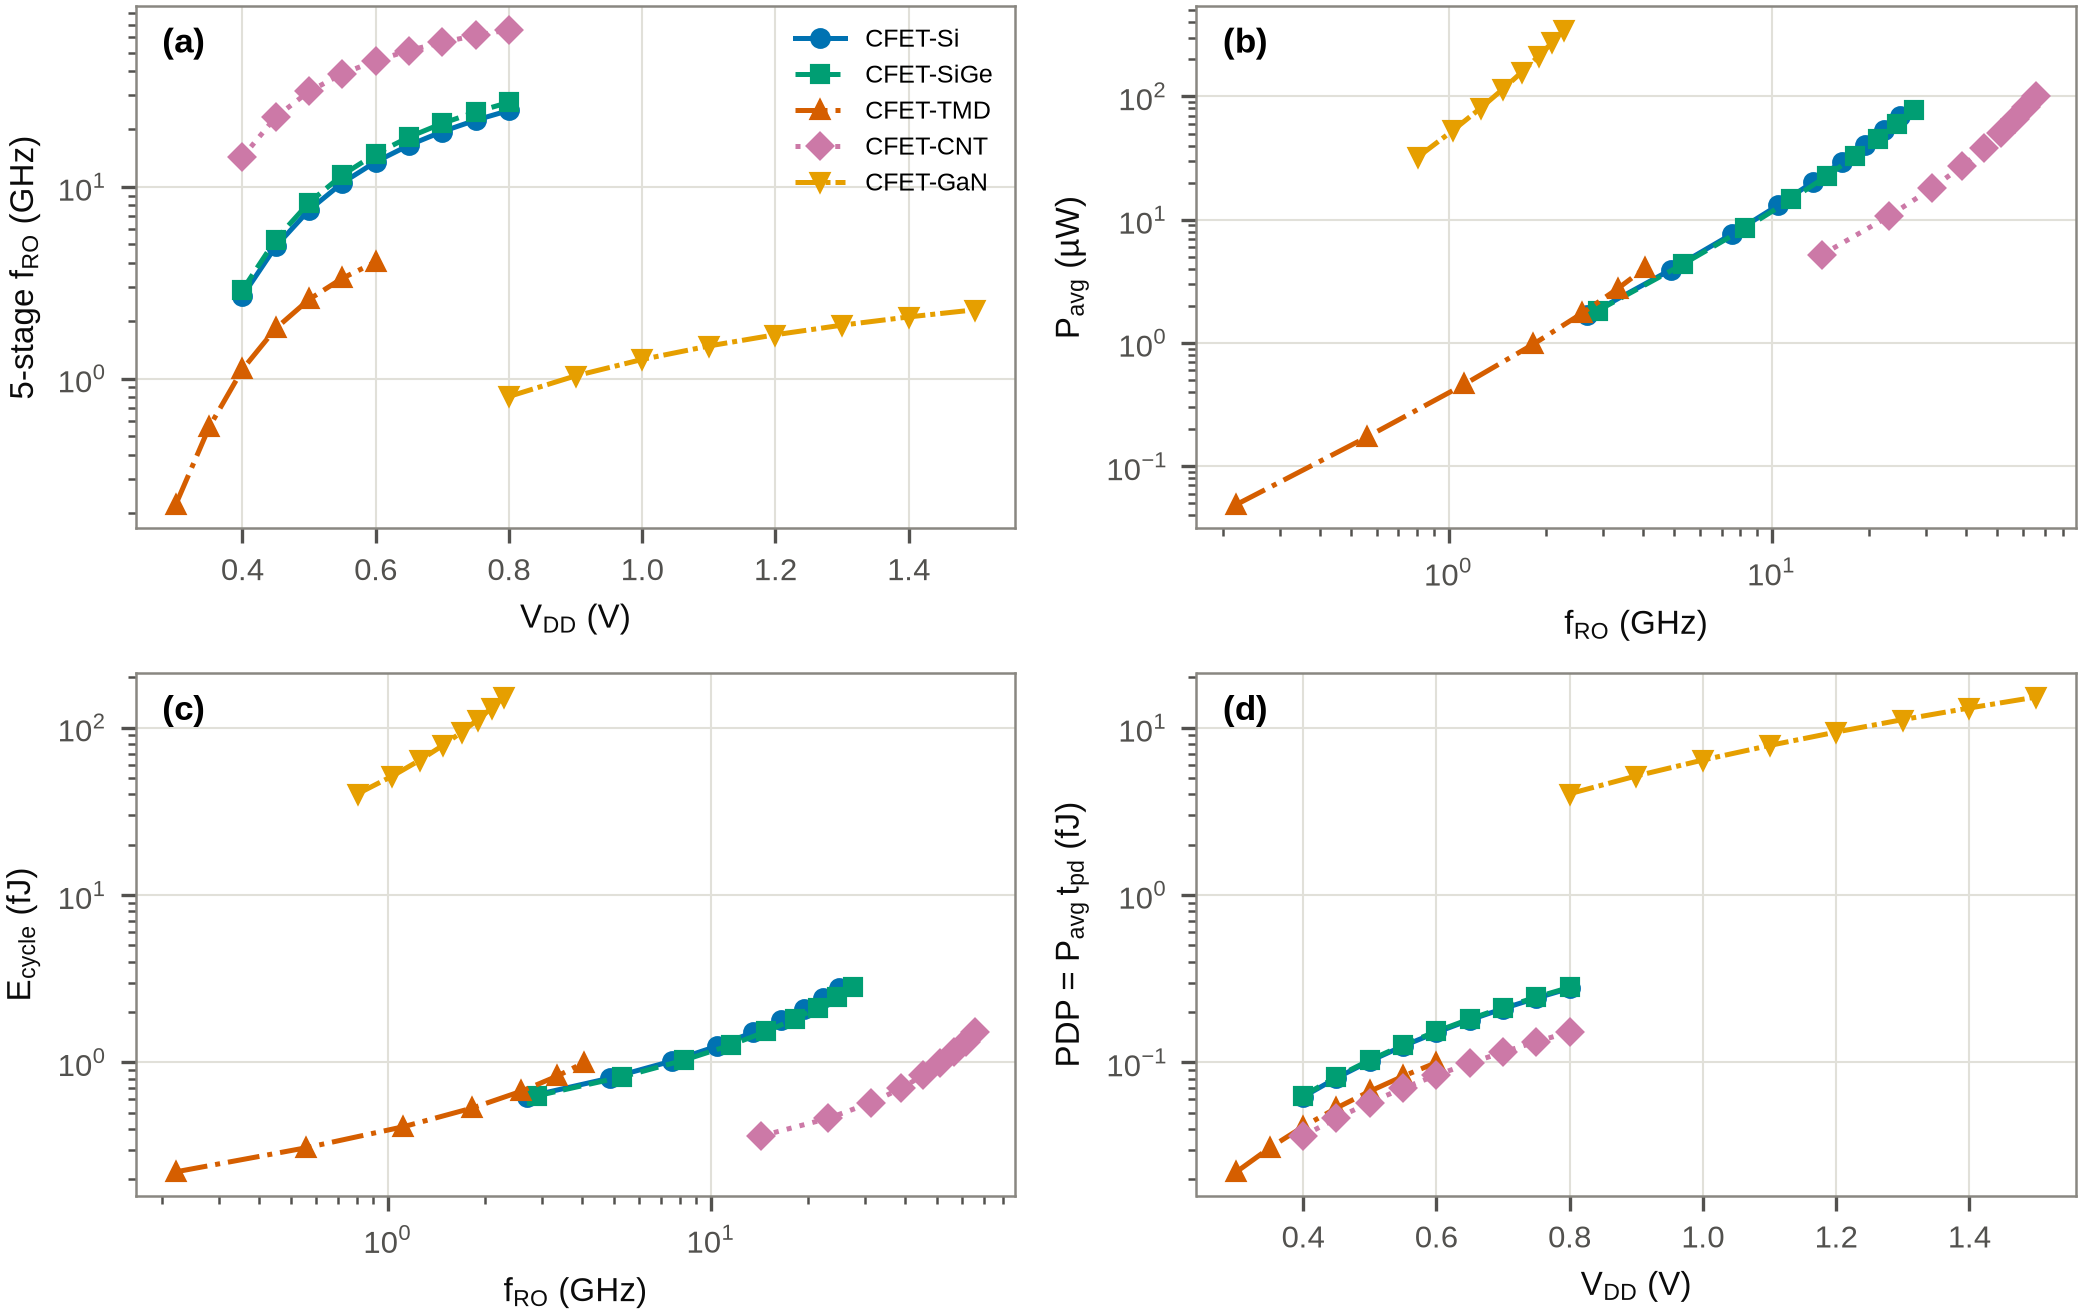
\includegraphics[width=\textwidth,height=0.82\textheight,keepaspectratio]{fig08_vdd_sweep.png}
\par\vspace{6pt}\noindent\textbf{Fig.~10.} Unified $V_{DD}$ sweeps of the 5-stage ROs: (a) $f_{RO}$ vs. $V_{DD}$, (b) power vs. frequency, (c) energy per cycle vs. frequency, (d) PDP vs. $V_{DD}$.
\end{figure}\clearpage
\begin{figure}[p]\centering
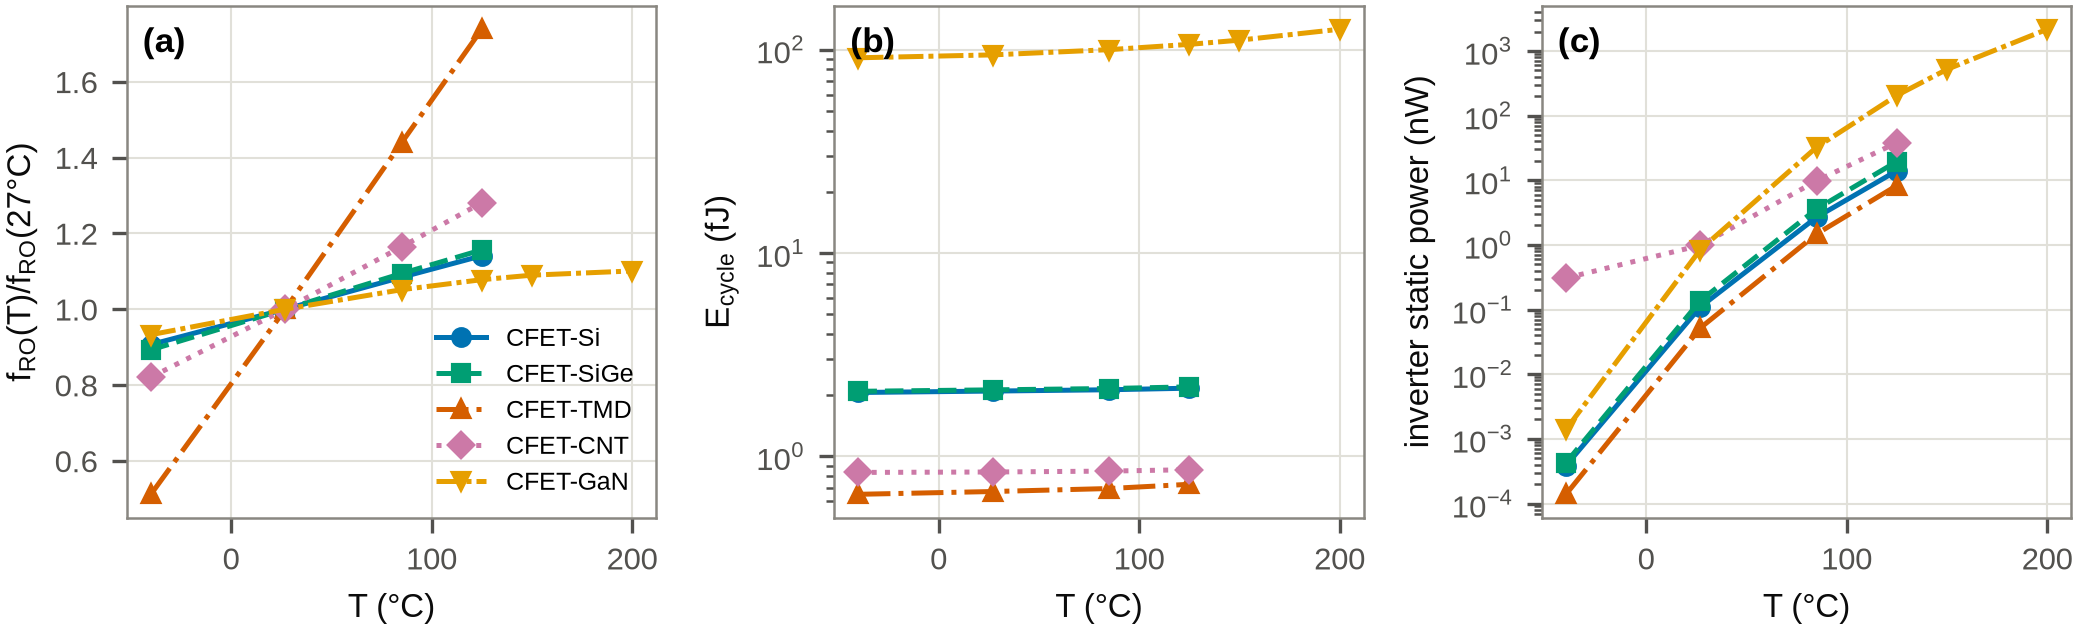
\includegraphics[width=\textwidth,height=0.82\textheight,keepaspectratio]{fig09_temperature.png}
\par\vspace{6pt}\noindent\textbf{Fig.~11.} Temperature sweeps at nominal $V_{DD}$ ($-40$ to 125$^\circ$C, GaN to 200$^\circ$C): (a) normalised $f_{RO}$, (b) energy per cycle, (c) inverter static power.
\end{figure}\clearpage
\begin{figure}[p]\centering
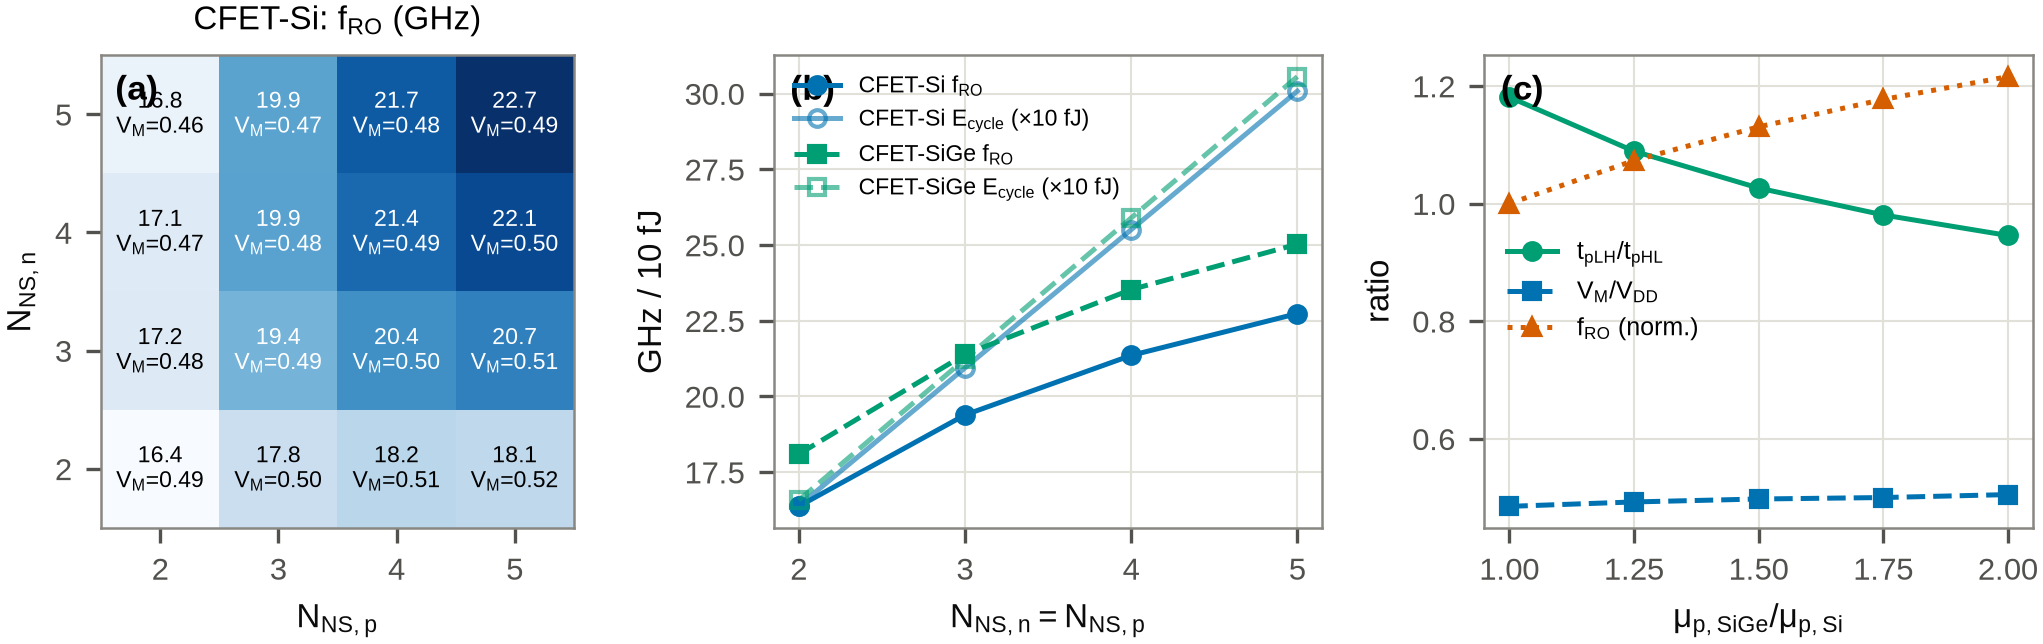
\includegraphics[width=\textwidth,height=0.82\textheight,keepaspectratio]{fig10_si_sige_sensitivity.png}
\par\vspace{6pt}\noindent\textbf{Fig.~12.} Si/SiGe study: 5-stage $f_{RO}$ and $V_M/V_{DD}$ vs. the number of nanosheets in the n- and p-tier for (a) CFET-Si and (b) CFET-SiGe; (c) effect of the SiGe/Si hole-mobility ratio on the rise/fall delay mismatch, $V_M$ and $f_{RO}$.
\end{figure}\clearpage
\begin{figure}[p]\centering
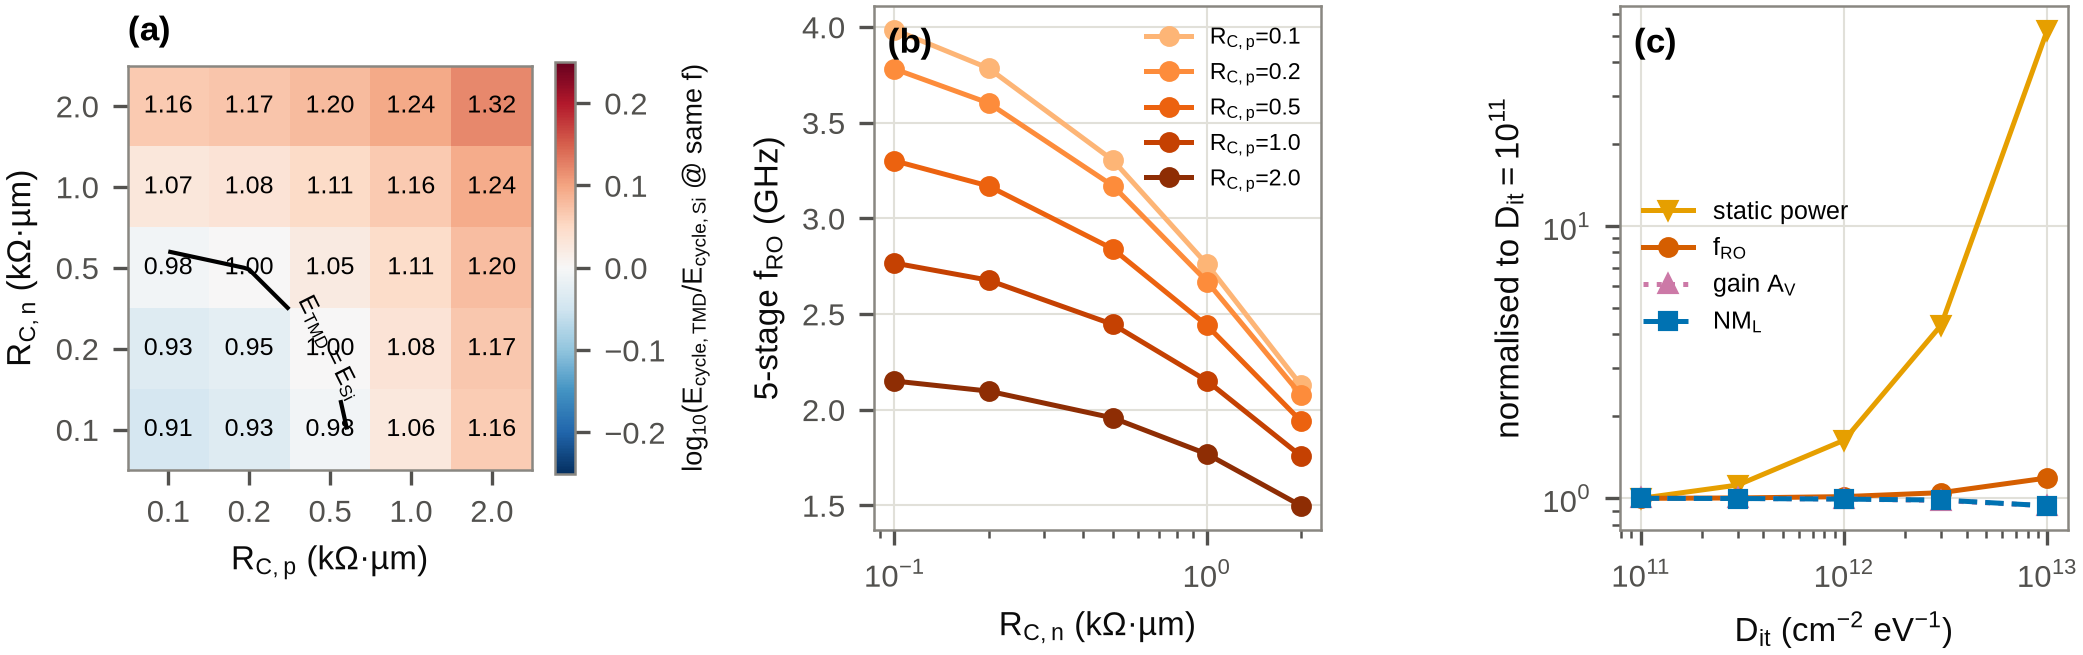
\includegraphics[width=\textwidth,height=0.82\textheight,keepaspectratio]{fig11_tmd_contact_crossover.png}
\par\vspace{6pt}\noindent\textbf{Fig.~13.} TMD study: (a) iso-frequency energy-per-cycle ratio $E_{TMD}/E_{Si}$ vs. the n- and p-contact resistance (the Si energy is interpolated at the TMD frequency from the Si $V_{DD}$ sweep extended to 0.3~V); (b) $f_{RO}$ vs. $R_{C,n}$; (c) effect of the interface trap density.
\end{figure}\clearpage
\begin{figure}[p]\centering
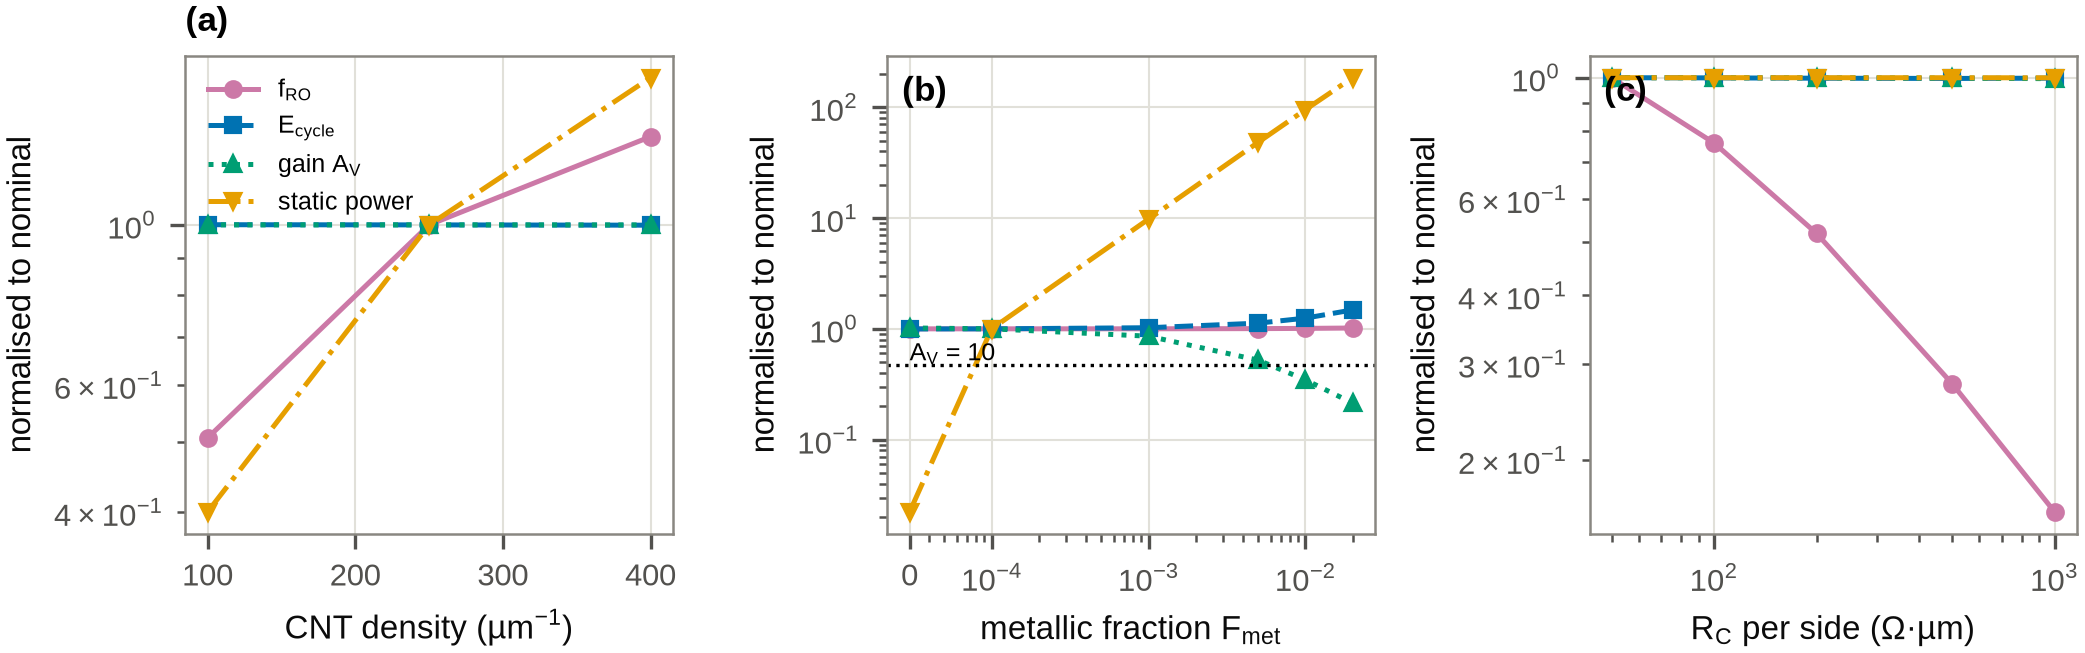
\includegraphics[width=\textwidth,height=0.82\textheight,keepaspectratio]{fig12_cnt_sensitivity.png}
\par\vspace{6pt}\noindent\textbf{Fig.~14.} CNT study: normalised $f_{RO}$ and PDP (left axes) and inverter static power (right axes) vs. (a) tube density, (b) metallic-tube fraction, (c) contact resistance.
\end{figure}\clearpage
\begin{figure}[p]\centering
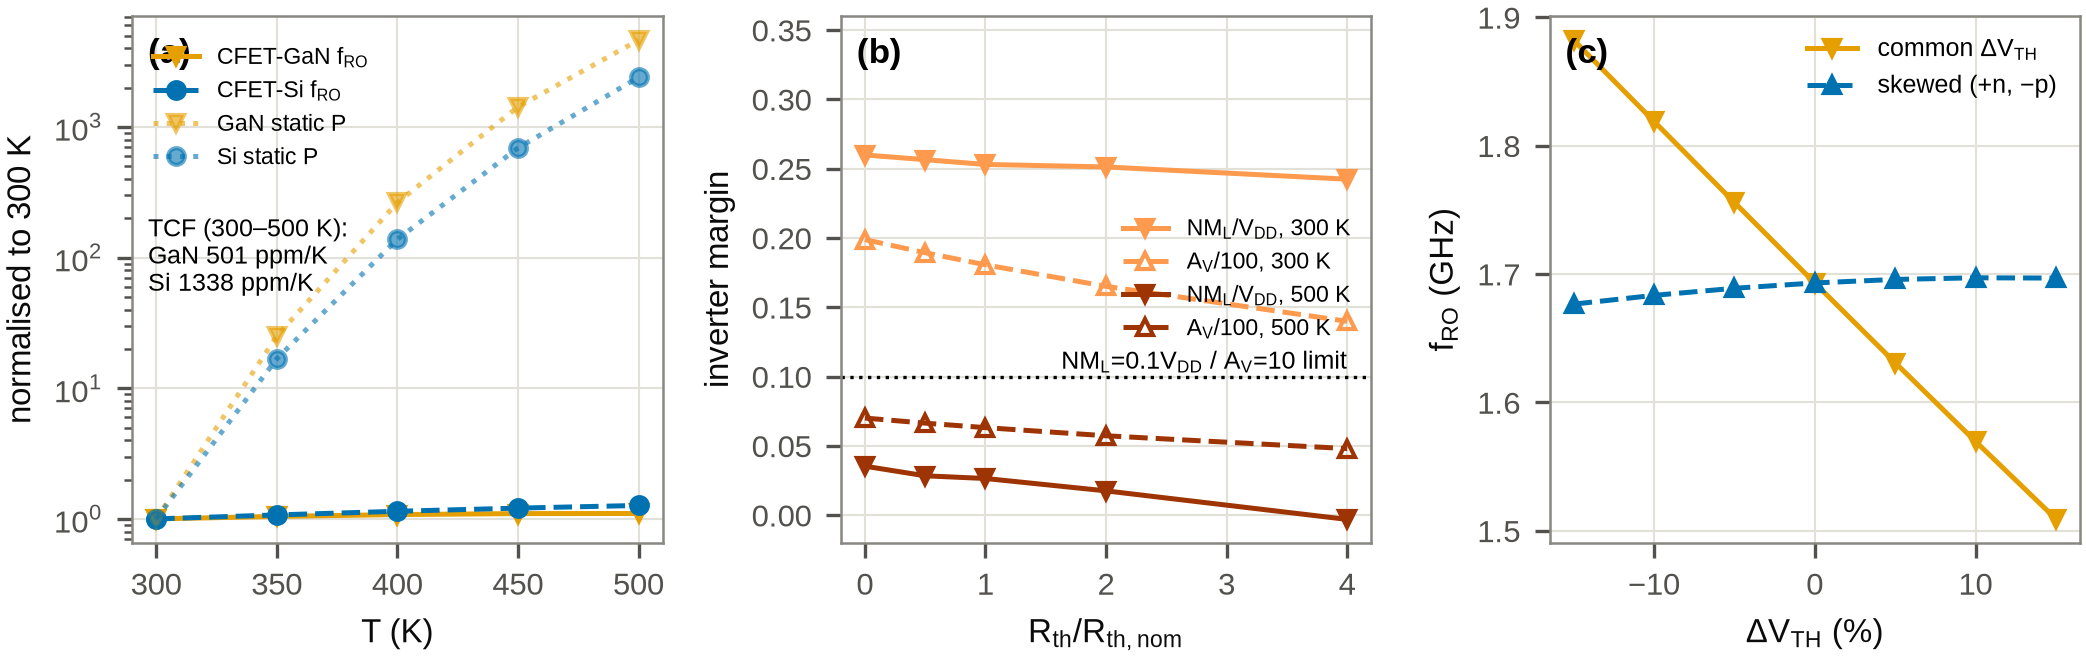
\includegraphics[width=\textwidth,height=0.82\textheight,keepaspectratio]{fig13_gan_thermal.png}
\par\vspace{6pt}\noindent\textbf{Fig.~15.} GaN study: (a) $f_{RO}$ and static power of CFET-GaN and CFET-Si from 300 to 500~K; (b) self-heating delay penalty vs. thermal resistance at three temperatures; (c) $f_{RO}$ vs. common and skewed threshold-voltage shifts.
\end{figure}\clearpage
\begin{figure}[p]\centering
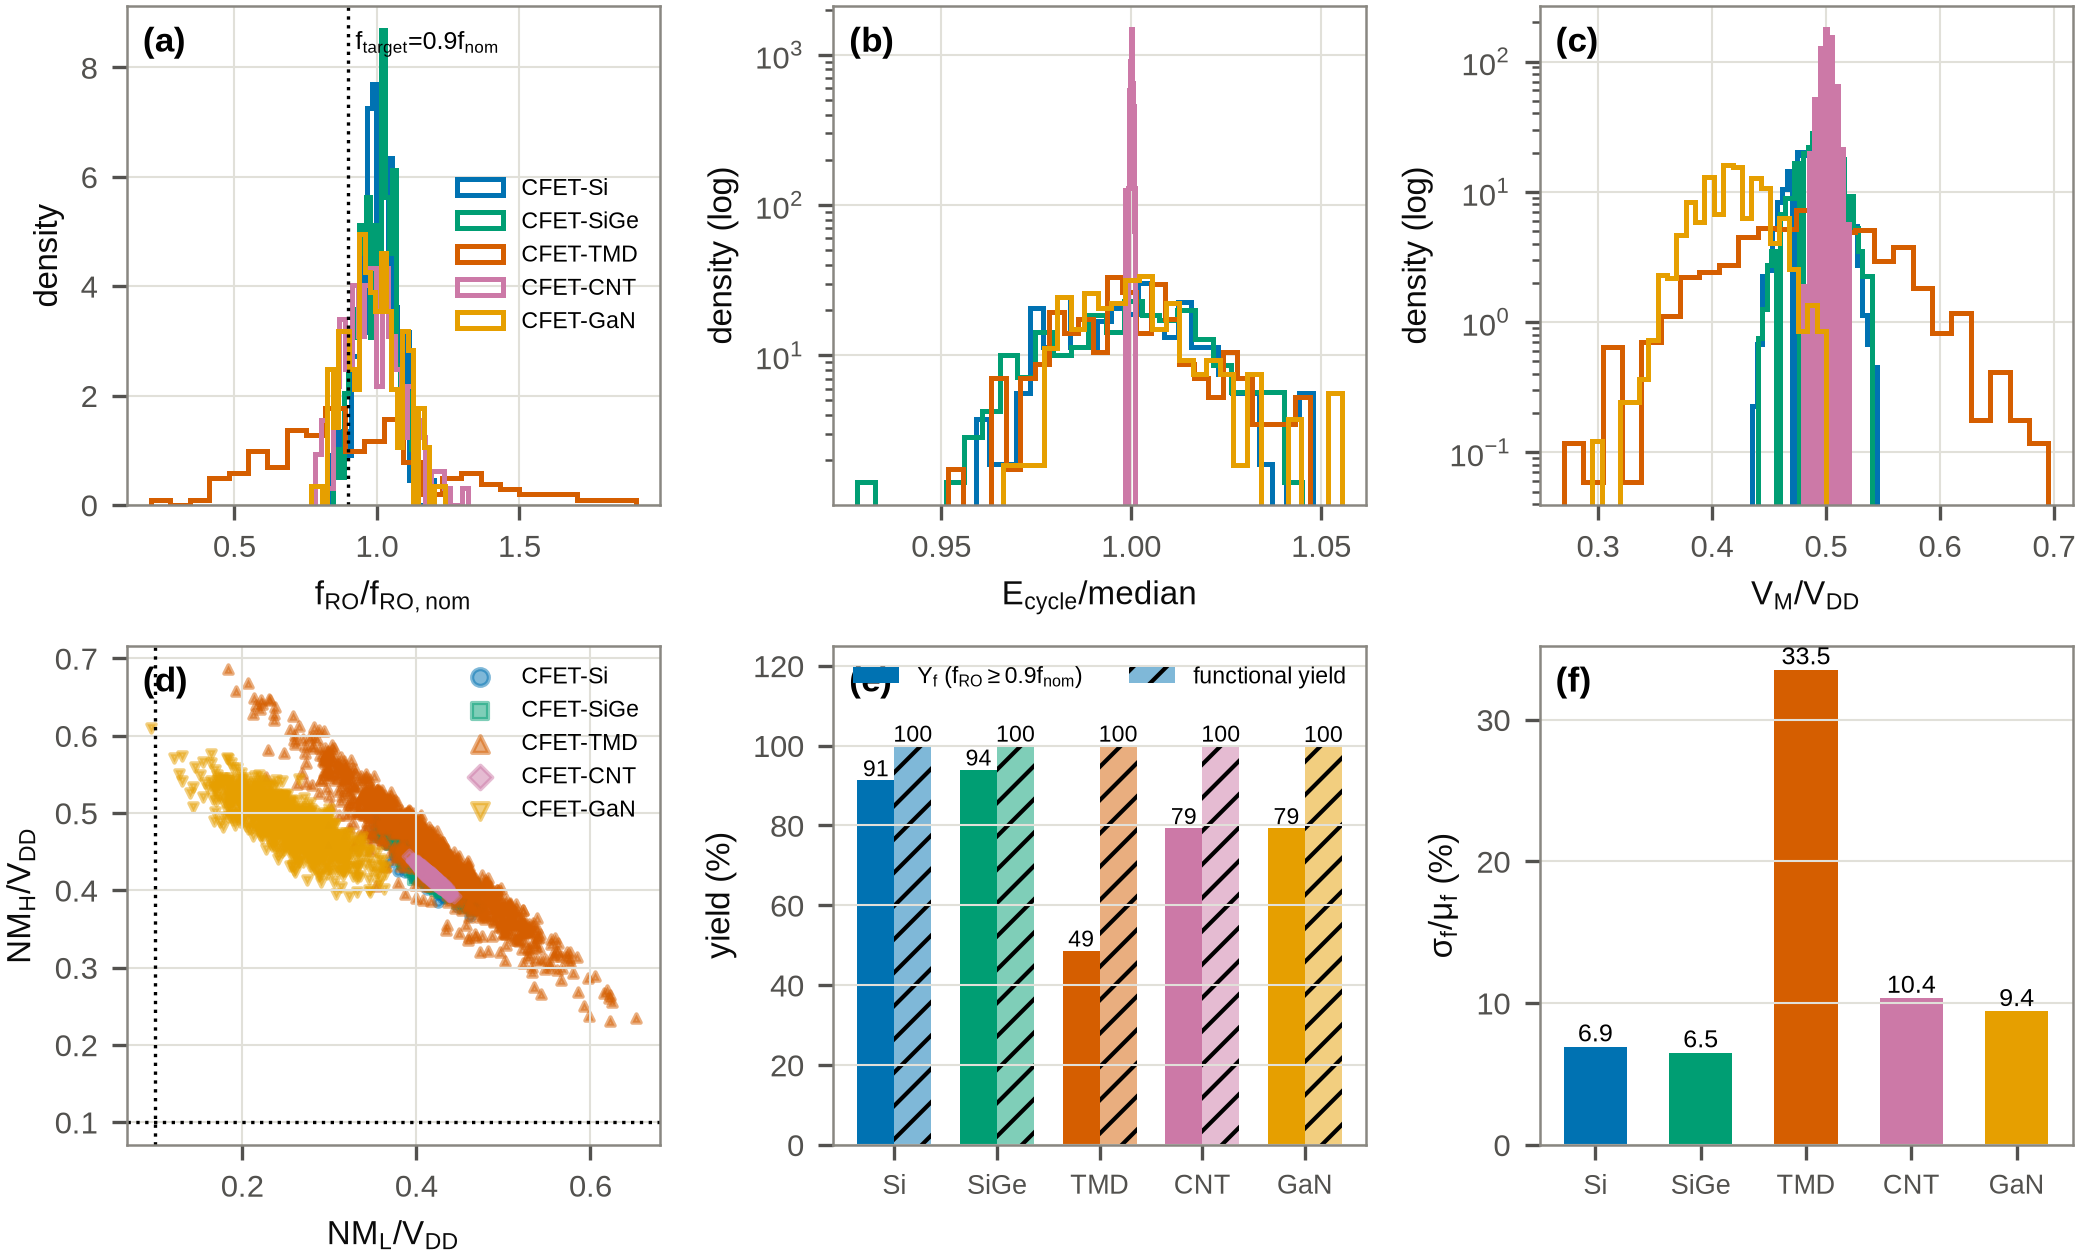
\includegraphics[width=\textwidth,height=0.82\textheight,keepaspectratio]{fig14_montecarlo.png}
\par\vspace{6pt}\noindent\textbf{Fig.~16.} Monte Carlo (200 RO samples and 1000 inverter samples per platform): (a) $f_{RO}$ normalised to nominal, (b) energy per cycle normalised to its median, (c) $V_M/V_{DD}$, (d) noise-margin scatter with the $0.1V_{DD}$ functional limits, (e) frequency yield $Y_f$ and functional yield, (f) relative frequency spread.
\end{figure}\clearpage
\begin{figure}[p]\centering
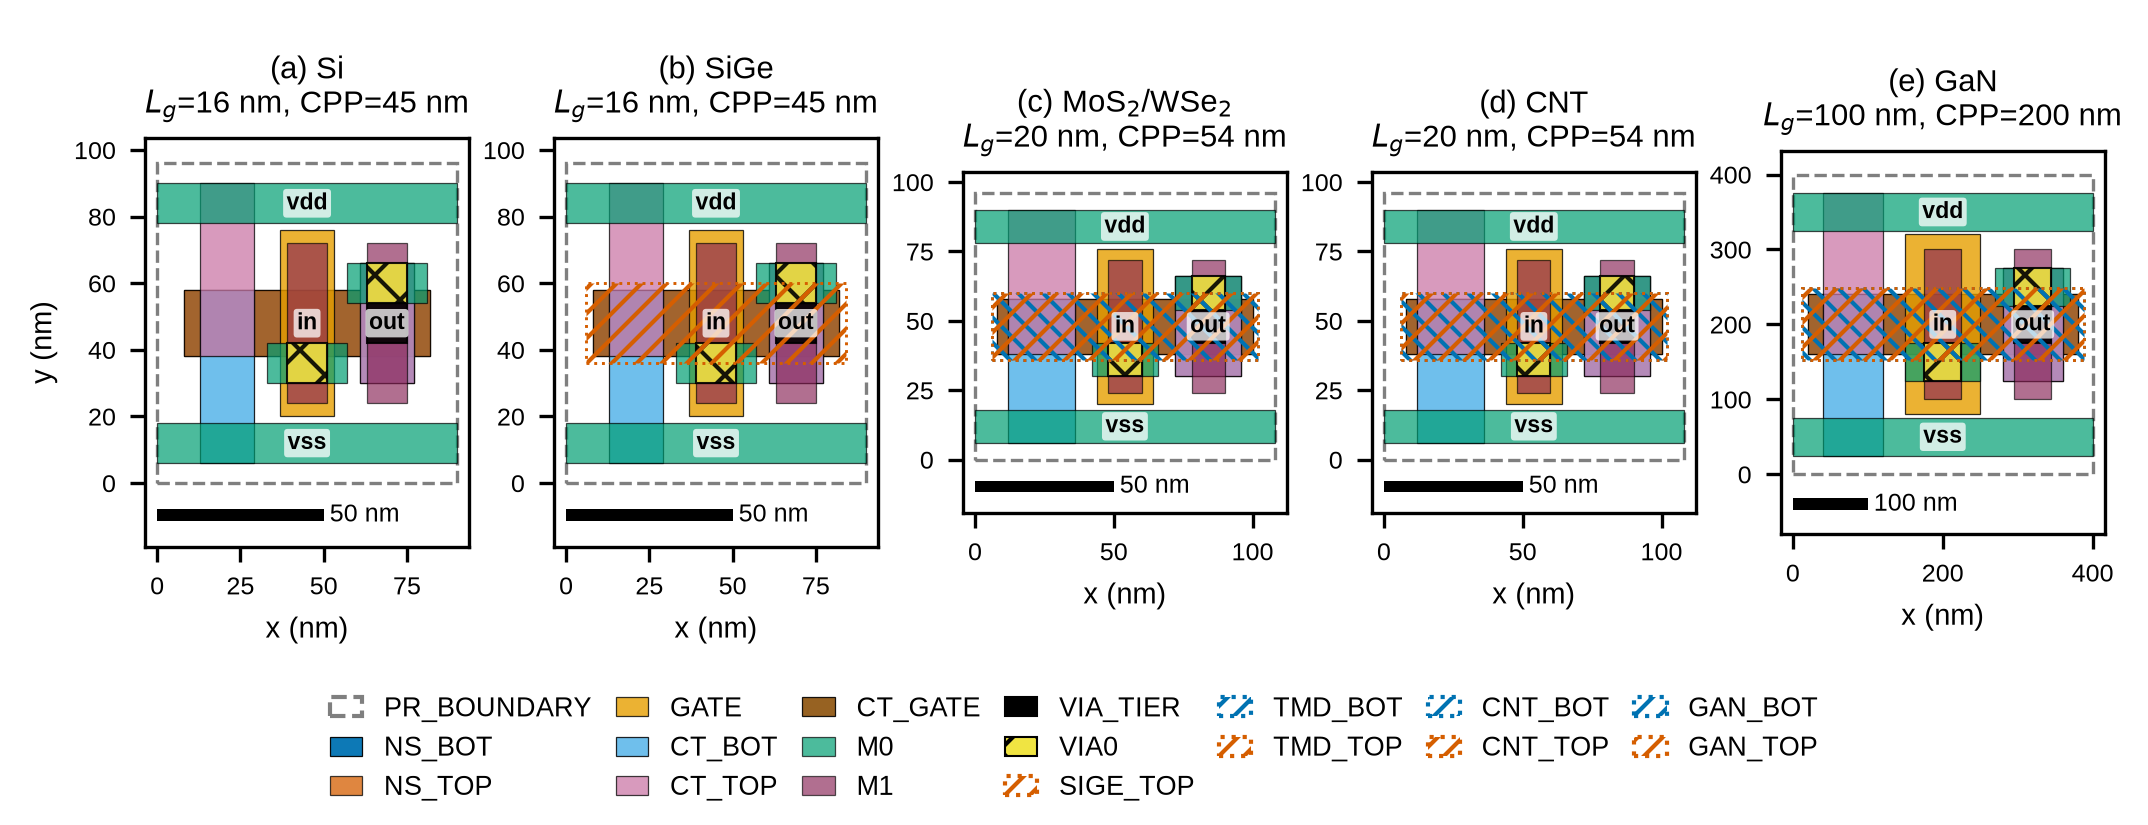
\includegraphics[width=\textwidth,height=0.82\textheight,keepaspectratio]{fig_layout_inverters.png}
\par\vspace{6pt}\noindent\textbf{Fig.~17.} Conceptual, DRC-clean GDSII layouts of the five CFET inverter cells (plan view; tiers drawn as separate layers): Si and SiGe at $L_g=16$~nm, CPP = 45~nm, 90$\times$96~nm cell; TMD and CNT projected at $L_g=20$~nm, CPP = 54~nm; GaN projected at $L_g=100$~nm, CPP = 200~nm.
\end{figure}\clearpage
\begin{figure}[p]\centering
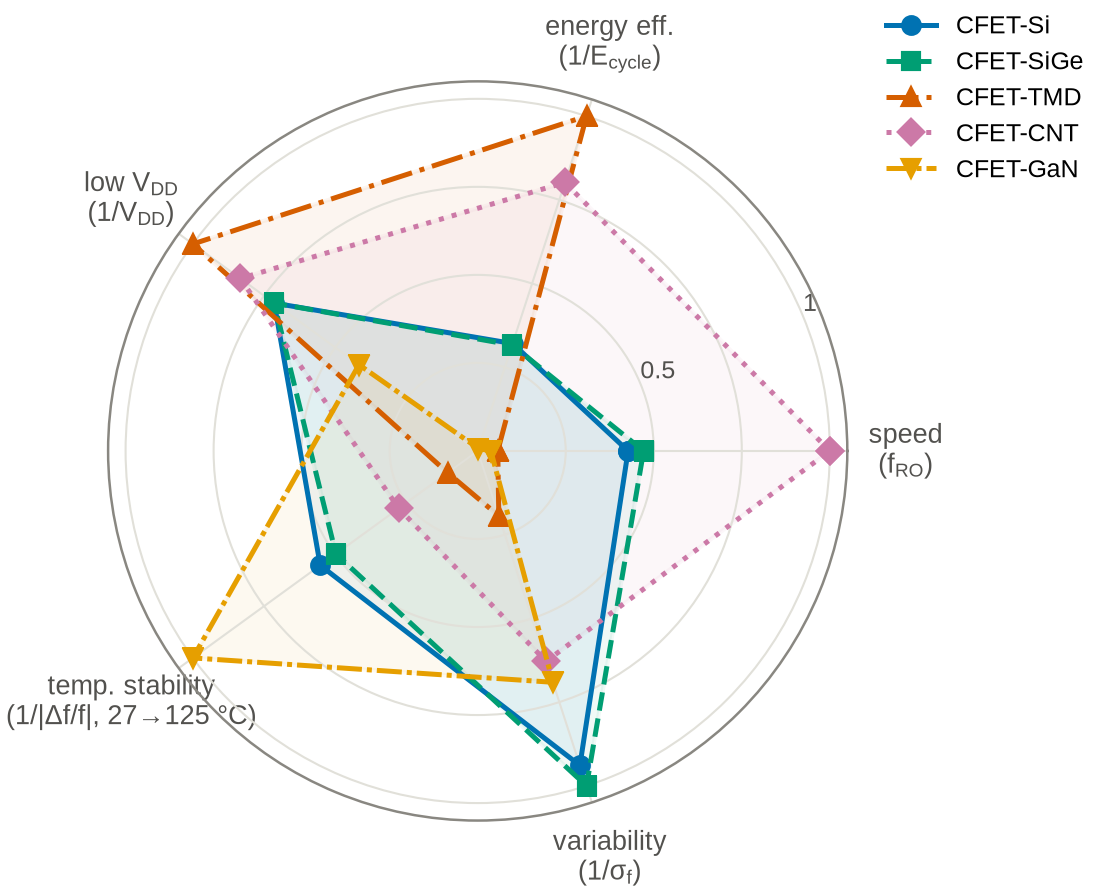
\includegraphics[width=\textwidth,height=0.82\textheight,keepaspectratio]{fig15_selection_chart.png}
\par\vspace{6pt}\noindent\textbf{Fig.~18.} Material-selection chart: speed, energy efficiency, low-$V_{DD}$ capability, temperature stability ($1/|\Delta f/f|$ between 27 and 125$^\circ$C) and variability ($1/\sigma_f$), each normalised to the best platform.
\end{figure}\clearpage
\end{document}
